% ****** Start of file aipsamp.tex ******
%
%   This file is part of the AIP files in the AIP distribution for REVTeX 4.
%   Version 4.1 of REVTeX, October 2009
%
%   Copyright (c) 2009 American Institute of Physics.
%
%   See the AIP README file for restrictions and more information.
%
% TeX'ing this file requires that you have AMS-LaTeX 2.0 installed
% as well as the rest of the prerequisites for REVTeX 4.1
%asd
% It also requires running BibTeX. The commands are as follows:
%
%  1)  latex  aipsamp
%  2)  bibtex aipsamp
%  3)  latex  aipsamp
%  4)  latex  aipsamp
%
% Use this file as a source of example code for your aip document.
% Use the file aiptemplate.tex as a template for your document.
\documentclass[%
9pt,
 aip,
%jmp,%
%bmf,%
%sd,%
rsi,%
 amsmath,amssymb,
preprint,%
%reprint,%
%author-year,%
%author-numerical,%
]{revtex4-1}

\usepackage{graphicx}% Include figure files
\usepackage{dcolumn}% Align table columns on decimal point
\usepackage{bm}% bold math
%\usepackage[outdir=./plots/]{epstopdf}


% \usepackage[utf8]{inputenc}
% \usepackage{amssymb,amsmath}
 % \usepackage{diagbox}
% \usepackage{tabularx}
% \usepackage{xcolor}
 \graphicspath{ {plots/} }
 %\DeclareGraphicsExtensions{.}

%\usepackage[mathlines]{lineno}% Enable numbering of text and display math
%\linenumbers\relax % Commence numbering lines

% %%%%%%%%%%%%%%%%%%%%%%%%%%%%%%%%%%%%%%%%%%%%%%%%%%%%%%%%%%%%%%%%%%%%%%%%%%
% % Karin: Egor, this helps me to interact with you in the manuscript
% % you may find
% %   \InTextCommment{KZ}{my comment}
% %   \todo{what to do}
% % FOR AUTHORS COMMENTS! REMOVE FROM HERE.....

% %\usepackage{multicol}
% %\setlength{\columnsep}{1cm}

 \usepackage[export]{adjustbox}
 \usepackage{ulem}
 \usepackage{anyfontsize}
 \usepackage[textwidth=1.2cm,textsize=tiny]{todonotes}
 \setlength{\marginparwidth}{1cm}

% % long comment
 \newcommand{\InTextComment}[2]{
 	%\renewcommand{\baselinestretch}{1.0} 
 	\textcolor{blue}{\textsf{{\footnotesize \textbf{- #1:} #2 -}}}\newline
 	%\renewcommand{\baselinestretch}{1.5} 
 }
 
% % UP TO HERE, BEFORE SUBMISSION
% %%%%%%%%%%%%%%%%%%%%%%%%%%%%%%%%%%%%%%%%%%%%%%%%%%%%%%%%%%%%%%%%%%%%%%%%%%

% KZ: activate for aiding reading
%\usepackage{helvet}
%\renewcommand{\familydefault}{\sfdefault}
%\fontsize{8}{11}\selectfont
\renewcommand{\baselinestretch}{1.2} %2.0

%defining dimensions

\newcommand{\thermalconductivity}{$\mathrm{W m^{-1} K^{-1}}$}
\newcommand{\hcoefficient}{$\mathrm{W m^{-2} K^{-1}}$}
\newcommand{\mobility}{$\mathrm{m^{2} V^{-1} s^{-1}}$}

\begin{document}

\preprint{aip}

 
\title[Heat transport in OLEDs]{Impact of thermal transport parameters on the operating temperature of OLEDs}

\author{G. Krikun}
\affiliation{ 
Institute of Solid State Physics and NAWI Graz, Graz University of Technology, Graz, 8010, Austria%\\This line break forced with \textbackslash\textbackslash
}%
  %\altaffiliation[Also at ]{Physics Department, XYZ University.}%Lines break automatically or can be forced with \\
\author{K. Zojer}%
 \email{karin.zojer@tugraz.at}
\affiliation{ 
Institute of Solid State Physics and NAWI Graz, Graz University of Technology, Graz, 8010, Austria%\\This line break forced with \textbackslash\textbackslash
}%

%\author{C. Author}
 %\homepage{http://www.Second.institution.edu/~Charlie.Author.}
%\affiliation{%
%Second institution and/or address%\\This line break forced% with \\
%}%

\date{\today}

\begin{abstract}
%Organic light emitting diodes (OLEDs) are developing perspective technology which already has its place in the screen market, taking over LCD screens.
%There exists another applications which are not yet commercialized, for instance, lighting.
%The amount of heat produced and dissipated in organic light emitting diodes (OLEDs) during the operation has a decisive impact on the degradation and on the homogeneiety of the brightness of large area OLEDs.
Excess heat in organic light emitting diodes (OLEDs) that is produced during their operation may accelerate their degradation and may cause an inhomogeneous brightness distribution, in particular in large area OLEDs.
%
%Utilizing OLEDs for lighting requires a homogeneous operation across large areas.
%Frequently encountered inhomogeneous brightness distributions often relate to non-uniform current-density and temperature distributions in the device.
%which is not always the case due to device self heating.
Assessing the quantitative impact of heat excess is difficult, because the electrical performance is governed by thermally activated charge transport and radiative recombination; 
%Assessing the quantitative impact of heat excess is difficult, because thermal and charge transport are strongly coupled in the organic semiconducting layers. 
%While the electrical performance is governed by thermally activated charge transport and radiative recombination, enhanced currents cause more Joule heating and non-radiative recombination.
electric currents that are elevated due to larger temperatures cause additional Joule heating and increase non-radiative recombination.
%Due to the peculiar coupling between thermal and charge transport in organics, the properties cannot be straight-forwardly decoupled.
%
This strong interdependence of thermal and charge transport implies that heating and the temperature distribution inside the OLED must be accounted for to reach a desired electrical performance or luminance. 
%Here we present a three-dimensional drift-diffusion model that self-consistently couples charge and heat transport. 
%Using simulations based on this model, we establish how parameters responsible for heat transport, i.e., the thermal conductivity of the organic layers and (ii) the heat transfer coefficient between the device surface and the environment govern 
%the 
Here we establish how parameters responsible for heat transport, i.e., the thermal conductivity of the organic layers and the heat transfer coefficient between the device surface and the environment govern the temperature inside the OLED. 
%We reveal the role of these parameters with simulations relying on a  three-dimensional drift-diffusion model that self-consistently couples charge and heat transport. 
To properly account for the interdependence of the electric current and the device temperature, we utilize simulations based on a three-dimensional drift-diffusion model that self-consistently couples charge and heat transport. 
%Using simulations based on this model, we establish how parameters responsible for heat transport, i.e., the thermal conductivity of the organic layers and (ii) the heat transfer coefficient between the device surface and the environment govern the .
%Within this model, there are 2 different parameters responsible for heat transport, namely (i) the thermal conductivity of the organic layers and (ii) the heat transfer coefficient between the device surface and the environment.
%
We establish that the heat transfer coefficient is able to compensate device heating much more efficiently than the thermal conductivity of the organic layers. 
Intentionally elevated operating temperatures, that may improve the OLEDs electric performance, are not necessarily beneficial, as any increase in operating temperature decreases the device stability. 
The thermal conductivity of organic layers is not a bootleneck for heat transport, because the encountered layer thicknesses in realistic device geometries prevent heat accumulation. 
The thermal effects being decisive for the OLED temperature occur in device layers beyond the electrically active region, i.e., in the layers that are not responsible for charge transport. 
We propose analytical expressions that relate the temperature in the device for a given point of operation to the heat transfer to the environment and the substrate.
%Valid PACS numbers may be entered using the \verb+\pacs{#1}+ command.
\end{abstract}

\pacs{Valid PACS appear here}% PACS, the Physics and Astronomy
                             % Classification Scheme.
\keywords{organic light emitting diode, operating temperature, heat transport, drift diffusion}%Use showkeys class option if keyword
                              %display desired
\maketitle


% \begin{quotation}
% The ``lead paragraph'' is encapsulated with the \LaTeX\ 
% \verb+quotation+ environment and is formatted as a single paragraph before the first section heading. 
% (The \verb+quotation+ environment reverts to its usual meaning after the first sectioning command.) 
% Note that numbered references are allowed in the lead paragraph.
% %	
% The lead paragraph will only be found in an article being prepared for the journal \textit{Chaos}.
% \end{quotation}

\section{Introduction}
%\thermalconductivity
%\hcoefficient
Two major factors presently hinder the application of organic light emitting diodes (OLEDs) for large-area lighting applications: device degradation and inhomogeneous light emission from the exterior surface.\cite{Park2011}
Both factors strongly relate to excess heat that is generated during operation.
On the one hand, elevated temperatures inside the OLEDs accelerate degradation,\cite{Xu2004,Zhou2000,Nenna2007} alongside with other factors such as water penetrating into the device \cite{Li2016}, surface roughness, and mass diffusion of material.
On the other hand, local variations in temperature and, hence, in the in-plane current density give rise to an inhomogeneous brightness distribution.\cite{Garditz2007,Kohari2013} 
% formulate!
% Such locally elevated current densities and temperatures originate, at least in part, from the available driving voltages that differ due to position-dependent ohmic losses in the large area contacts .\cite{Fischer2014} 
The primary origin of such locally elevated current densities and temperatures are non-uniformly distributed driving voltages, because these voltages differ due to position-dependent ohmic losses in the large area contacts.\cite{Fischer2014} 
%A common origin for inhomogeneous current densities is are effective driving voltages across a that strongly vary due to 
As a consequence, the efficiency of how heat is dissipated from the device becomes dependent on the position in which the heat is generated. 
%Excess heat that remains in the device is prone to promote device degradation and to lower the lifetime.\cite{Xu2004,Zhou2000,Nenna2007}
%These effects and their consequences for device performance are \cite{Fischer2014}. 
Even if heating is compensated by heat outflow,\cite{Park2014} such instabilities may lead to local "bright spots" in which the device will degrade much faster.

The quantitative impact of heat excess is particularly difficult to assess, because the major effects that govern the electrical performance are thermally activated, i.e., the charge transport and the recombination efficiency in the organic layers. 
An increasing temperature enlarges the charge carrier mobility in organic thin films\cite{Bassler1993} and the recombination rates and, hence, increases the device current. In turn, this enhanced current causes larger Joule heating and elevates the temperature even further.
If this process of self-activated heating is balanced by a sufficient outflow of heat, the current reaches a stable steady state. 
Unbalanced, the self-activated heating process can drive the device into a ''vicious cycle'', which will eventually overheat the device to the point where it is not operable anymore.


%Brightness inhomogeneity can be treated by conductive mesh grid, which makes voltage on the transparent contact more smooth \cite{Park2012}.\textcolor{red}{ Nevertheless, this solution makes still quite expensive (compared to analogs on lighting market) device more sophisticated and more expensive.}

%In this article, we assess how the parameters that govern heat transport in OLEDs promote heat dissipation, see Fig. \ref{fig:bcpic}.
%In this article, we assess how the parameters that are responsible heat transport in OLEDs govern the temperature distribution in the device. 
In this article, we pursue the question how the parameters that are responsible for heat transport in OLEDs govern the temperature distribution in the device.
% In analogy to the vast optimization efforts spent to unravel the most favorable conditions regarding the electric properties of OLEDs, we will particularly focus on the following aspects related to the thermal properties of OLEDs:
% In particular, we focus on the thermal properties that most favorably support the device operation - in analogy to the vast optimization efforts spent to unravel the most favorable material properties for charge transport.
Inspired by the vast efforts spent to optimize the material properties for charge transport, our article focuses on the \textit{thermal properties} that most favorably support the device operation. 
Specifically, we seek to learn (i) whether the parameters that govern heat transport represent separate tuning handles to dissipate heat, and (ii) with which layers of the OLED stack the heat dissipation can be efficiently controlled.
% (i) Are $\kappa$ and $h$ separate tuning handles to dissipate heat?
% (ii) With which layers of the OLED stack can the heat dissipation be efficiently controlled?
%(iii) Can we identify a relation between the device temperature, the electric current, and the heat transport parameters?
As further asset we seek to determine a relation between the device temperature, the electric current, and the heat transport parameters.
With such a relation, even if approximate, we would be able to predict how the OLED operation is affected by its thermal transport properties and able to estimate the impact of heat dissipation directly from an experimentally obtained current voltage characteristics.

\begin{figure}
    \centering	
    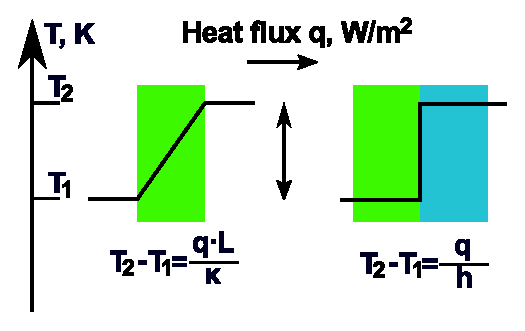
\includegraphics{new_bc.eps}
    \caption{ Schematic illustration of the thermal conductivity $\kappa$ (left) and the thermal transport coefficient $h$ (right). Without heating in the layer, the thermal conductivity $\kappa$ is the coefficient of proportionality between a heat flux $q$ and the temperature gradient $T_2 - T_1$ (Fourier law), $L$ denotes the thickness of the layer. For a heat flux $q$ across an interface formed by two materials, the heat transfer coefficient $h$ determines the difference between the temperatures on each side of device.}
    \label{fig:bcpic}
\end{figure}

As a first parameter, we consider the thermal conductivity $\kappa$ of individual organic layers. 
As illustrated in Figure~\ref{fig:bcpic}, $\kappa$ describes how efficient heat is transported from the heat source through a layer of a thickness $L$. 
%
% There are clear indications that heat outflow from the device can be sufficiently improved by choosing appropriate substrate\cite{Chung2009,Triambulo2016}. This means that interface between border layers and ambient environment plays crucial role. Furthermore, while device performance depend on absolute temperature of organic layers, heating changes device temperature relative to the ambient temperature. Hence, ambient will influence device performance and we need a tool to decouple device thermal properties and ambient properties. 
% Therefore, we need to introduce interface between ambient and border layers into simulation tool. We are tackling this problem using second parameter, heat transfer coefficient $h$, which can be used to describe heat transport through the interface \cite{Jin2014}.  We are using this parameter to describe particular interfaces between ambient environment and the border layers of the device. 
The second considered parameter is the heat transfer coefficient $h$ that describes heat transport through an interface (Figure~\ref{fig:bcpic}).\cite{Jin2014}
In the context of OLEDs, the heat transfer coefficient between the outermost layers and the ambient environment  appears to be most crucial.
There are clear indications that the heat outflow from the device can be sufficiently improved by choosing an appropriate substrate.\cite{Chung2009,Triambulo2016} 
As the generated heat has to be dissipated with respect to ambient temperature, the absolute temperature within the organic layers will be influenced not only by the electric current, but also by the ambient temperature.
% Therefore, we need to introduce interface between ambient and border layers into simulation tool.   We are using this parameter to describe particular interfaces between ambient environment and the border layers of the device. 

%%In this article we intent to particularly reveal and, if applicable, to explain the following considerations.
%%In this article we inspect the interplay between charge and heat transport from the following angles:
%%In particular, our investigation is guided by the following key questions:
% In particular, we dedicate particular effort to address the following key questions:
% (i) Do $\kappa$ and $h$ assume distinct roles in the dissipation of heat?
% (ii) With which layers of the OLED stack can the heat dissipation be efficiently controlled?
% (iii) Can we identify a relation between the device temperature, the electric current, and the heat transport parameters? With such a relation, even if approximate, we would be able to explain how the OLED operation is affected by its thermal transport properties and able to estimate the impact of heat dissipation directly from an experimentally obtained current voltage characteristics.

%We appropriately account for the sequence of self-activated heating by employing drift-diffusion based simulations that simultaneously monitor charge and heat transport and establish a self-consistent feedback between them.
% To that aim, we explicitly monitor how these two types of parameters, i.e., $\kappa$ and $h$, contribute to the thermal and electric behavior of the OLED. 
% We appropriately account for the sequence of self-activated heating by employing drift-diffusion based simulations. 
We employ drift-diffusion based simulations to monitor how these two types of parameters, i.e., $\kappa$ and $h$, contribute to the thermal and electrical behavior of the OLED.
With such simulations, we simultaneously account for charge and heat transport based on the (i) geometry of the OLED stack, (ii) the material parameters governing the charge and the thermal transport, and (iii) the coupling between charge and heat transport to establish a self-consistent feedback between them.
This allows us to obtain current-voltage characteristics and temperature-voltage relation for an OLED that is operated at a given ambient temperature. 

% % While we were searching for optimal heat transport parameters, it turned out that thermal conductivities of organic layers are less important for the device performance than heat transfer coefficient $h$.  
% % In this article we put main effort to describe its influence, derive certain approximations which can be made to get better grasp on what is going on and to measure it in the experiment.





\section{Methodology}

To efficiently model the charge and heat transport, we distinguish between two device regions, i.e., (i) the region in which heat is generated, and (ii) in device regions, in which solely heat is transported. 
These regions are reflected in the schematic OLED cross section in Figure~\ref{fig:setup} as follows:
In the organic layers between the electric contacts, the electric current produces both Joule heating and heating due to non-radiative recombination. 
Hence, the region comprising the organic layers and the contacts will be described with a three dimensional drift-diffusion model for coupled charge and heat transport.
%, because heat will promote charge transport, while charge transport is the source of heat that is going to compete with heat dissipation.  
In the regions outside the contacts, i.e., in the encapsulation and substrate layers, no further heat is produced. 
%In the absence of electric current, only the heat transport equation remains to be solved. 
%Rather than solving the heat transport equation for the entire device with the same elaborate numerical setup, we directly employ the analytical solution with the heat generation profile within the organic layers as source term.
In the absence of electric current, it is sufficient to solve the heat transport equation.
The latter equation can be solved analytically for steady state operation, sparing us to solve the heat transport equation for the entire device with the  elaborate numerical approach necessary for the electrically active region.
For convenience, the OLED cross-section shown in Figure~\ref{fig:setup} is oriented such that the layers are stacked along the z-axis and laterally extended in the x-y plane.
In this orientation, the externally applied voltage shall be uniformly applied between cathode and anode, i.e., the voltage drops in z-direction and is uniform in x and y directions.

\begin{figure}
	\centering
    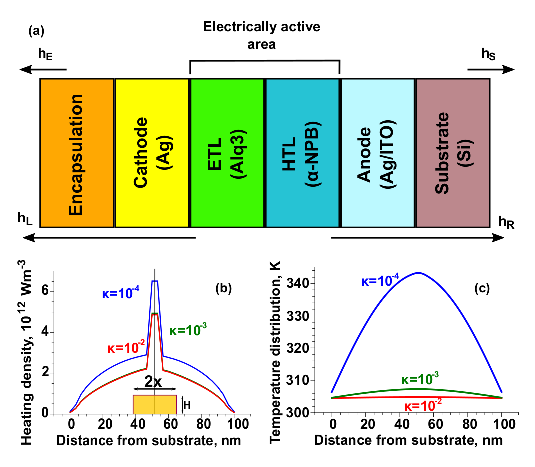
\includegraphics{General_plots_0.eps}
    \caption{(a) Schematic cross section of an OLED containing an electron and hole conducting layer sandwiched between two contacts. 
    Beyond these electrical contacts, an encapsulation layer and a substrate with their heat transfer coefficients to the ambient, $h_{\mathrm{E}}$ and $h_{\mathrm{S}}$, are considered. 
    Within the organic layers, the coupled charge and heat transport is self-consistently simulated with a drift-diffusion approach. 
    %Due to the absence of heat generation in the encapsulation layer and in the substrate, the heat propagation is considered by directly solving the heat transport equation. 
    %As a consequence, 
    The combined impact of heat transfer to the ambient, heat transfer between and through subsequent encapsulation or substrate layers can be lumped into an effective heat transfer coefficient %    
    $h_{\mathrm{L}}$ (encapsulation side) and $h_{\mathrm{R}}$ (substrate side), respectively.
    (b) Profile of the heat density distribution in a symmetric device between the electrical contacts that are separated by $L$=50~nm, no injection barrier,  $h$~=~$h_{\mathrm{L}}$~=~$h_{\mathrm{R}}$=~$10^{4.25}$~\hcoefficient, $\kappa=10^{-2}$(bottom)/$10^{-3}$(middle)/$10^{-4}$(top)~\thermalconductivity~ in each organic layer operated at room temperature $T$~=~300~K with $V$~=~5~V. 
    (c) Corresponding temperature distribution.}
\label{fig:setup}
\end{figure}


\subsection{Drift diffusion model} 
The drift-diffusion model is an established approach for the investigation of the electrical performance of OLEDs.\cite{Davids1998,Knapp2010,Knapp2011,Ruhstaller2003,Slawinski2011,VanMensfoort2008} 
% KZ: Can we justify it more elegantly?
%It is less precise than Monte-Carlo approach \cite{Mesta2013}, but allows to incorporate more effects into the device. 
Since the model describes transport processes with effective material parameters, the model can be straight-forwardly extended to consider also heat transport and thermoelectric effects.\cite{Park2011a}

All charge densities, energy densities, and material parameters are dependent on the position in the device, %
so that the fluxes of the thermal energy and charges are three component vectors.
Below we describe the formulation and the implementation of the fully three dimensional drift-diffusion model.
Such a consideration of three-dimensional fluxes and related density distributions is crucially required to address lateral variations in temperature and in-plane current densities. 
Hence, we are aiming at devising a simulation code with which one can address temperature-related inhomogeneity issues that are beyond the scope of this work. 

In general, charge and heat transport are governed by two types of equations, the continuity equations and the current density equations.
The continuity equations for the densities of mobile charges, i.e., of electrons, $n$, and holes, $p$, and the density of thermal energy, $\rho c_p T$, read:

\begin{subequations}
	\begin{gather}
		\frac{\partial p}{\partial t} - \mathrm{div}\left( \mathbf{j_p}\right) =G-R\label{eq:contp}\\	
		\frac{\partial n}{\partial t} - \mathrm{div}\left( \mathbf{j_n}\right)=G-R\label{eq:contn}\\
		\rho c_p \frac{\partial T}{\partial t}-\mathrm{div}\left(\mathbf{q_T}\right)=H\label{eq:contT}\qquad 
	\end{gather}
    \label{eq:cont}
\end{subequations}

Therein, $\mathbf{j_n}$ and $\mathbf{j_p}$ are the electron and hole flux (rather than the electric current densities) respectively, $G$ and $R$ the generation and recombination rates. We are using the Langevin recombination model.\cite{Langevin1903} 
Note that there are more refined models to account for recombination rates which, however, would introduce additional free parameters to the our description.\cite{Lee2014,VanDerHolst2009} 
In Eq.~\ref{eq:contT}, $T$ refers to the temperature, $\rho$ to the mass density, $c_p$ to the specific heat capacity, and  $\mathbf{q_T}$ to the heat flux.
The term $H$ accounts for the amount of heat energy added or abstracted per unit volume and per unit time. 
The current density equations connect the fluxes with the densities: 
\begin{subequations}
	\begin{gather}
		\mathbf{j_p}=\mu_p p \left(\mathbf{\nabla} \phi + S \mathbf{\nabla} T \right) - D_p \mathbf{\nabla} p \label{eq:ddjp} \\
		\mathbf{j_n}=-\mu_n n \left(\mathbf{\nabla} \phi + S \mathbf{\nabla} T \right) - D_n \mathbf{\nabla} n \label{eq:ddjn} \\
		\mathbf{q_T}=-\kappa \mathbf{\nabla} T\qquad \label{eq:fourierlaw}
	\end{gather}
    \label{eq:connectionDensitiesToFluxes}
\end{subequations}
Eqs.~(\ref{eq:ddjp},\ref{eq:ddjn}) contain the material parameters responsible for charge transport, i.e., $\mu_i$ is the mobility of the corresponding charge carriers, $D_i$ the diffusion constant, and $S$ the Seebeck coefficient. Eq.~(\ref{eq:fourierlaw}) formulates the Fourier law and contains the heat conductivity $\kappa$.
To account for the hopping nature of the transport in organic materials, we consider mobilities and a Seebeck coefficient that  depend on electric field, temperature, and charge carrier concentration. 
There are different methods to incorporate this dependencies,\cite{Fishchuk2010,Fishchuk2013} we use relations that were previously extracted from Monte Carlo simulations.\cite{Lu2015,Pasveer2005}

The current densities $\mathbf{j_p}$ and $\mathbf{j_n}$ across organic-organic heterojunctions are also treated with Eqs.~(\ref{eq:ddjp},\ref{eq:ddjn}).
%
Besides drift and diffusion, we introduce an additional driving force for electrons and for holes at the position of the heterojunction. 
The extent of this force reflects how the transport-relevant levels of the two organic materials align at the heterojunction.
We obtain this force from a generalized electrostatic potential, $\tilde{\phi}$, that contains two additional terms compared to the actual electrostatic potential $\phi$. 
% The first term accounts for the difference in the transport level energies $E_{\mathrm{HOMO}}$ and $E_{\mathrm{LUMO}}$ of the two materials joining at the heterojunction. 
% This term introduces an additional potential drop across the heterojunction between two adjacent positions, i.e., $\left( E_{\mathrm{HOMO}_1}-E_{\mathrm{HOMO}_2} \right)$ for holes and $\left( E_{\mathrm{LUMO}_1}-E_{\mathrm{LUMO}_2} \right)$ for electrons, respectively. \cite{Sutherland}
The first term accounts for the difference in the nominal transport level energies $E_{\mathrm{HOMO}}$ and $E_{\mathrm{LUMO}}$ of the two materials by introducing an additional potential drop across the heterojunction, i.e., $E_{\mathrm{HOMO}_1}-E_{\mathrm{HOMO}_2}$ for holes and $E_{\mathrm{LUMO}_1}-E_{\mathrm{LUMO}_2}$ for electrons, respectively.\cite{Sutherland}
The second term accounts for the fact that the density of states available for hopping transport is changing across the heterojunction.
We cast this change in the density of states into a local contribution to the generalized electrostatic potential following the argumentation in Ref.~\cite{Liemant}.
The current densities $\mathbf{j_p}$ and $\mathbf{j_n}$ entering and leaving the OLED across the contacts are described by a net injection current.
This injected current is a superposition of different contributions that are associated to the offset between the transport levels and the workfunction of the electrode metal, forming the injection barrier. We specifically consider current density contributions due to thermionic and tunneling injection (from contact into organic layer) as well as interface recombination (from organic layer into the contact).\cite{Davids1998a,Gruber2012,Scott1999}
The individual contributions are self-consistently determined as a function of the local situation present at each contact during operation. Particularly important are the temperature (thermionic injection) and the local electric field (thermionic and tunneling injection). 

The local electric field that drives the charges is given as the gradient $-\mathbf{\nabla}\phi$ of the electrostatic potential $\phi$. 
At heterojunctions, this field is replaced by an effective field $-\mathbf{\nabla}\tilde{\phi}$ related to the generalized electrostatic potential $\tilde{\phi}$. 
The potential $\phi$ is connected to the local net charge density via the Poisson equation 
\begin{equation}
    \epsilon_0 \mathbf{\nabla} \left( \epsilon_r \mathbf{\nabla} \phi \right) = q \left(n-p\right), \label{eq:poisson}
\end{equation}
in which $\epsilon_r$ is relative dielectric permittivity and $\epsilon_0$ the vacuum permittivity.
The potential set at the cathode corresponds to the applied voltage $V$, while the potential at the anode is set to zero. 

The heat flow $\mathbf{q_T}$ across the organic-organic heterojunction is considered in Eq.~(\ref{eq:fourierlaw}) via a thermal conductivity $\kappa$ that is averaged with respect to the $\kappa$ of the layers meeting at the interface.
The heat flow is directed out of the device, i.e., $\mathbf{q_T} = \mathbf{q}_z > 0$ at $z=L$,  if the temperature in the device exceeds the ambient temperature.
The heat flow out of the contacts, i.e., the flow leaving the region in which heat is generated, is assumed to be proportional to the difference in the temperature of the contact surface, e.g., at $z=L$, and the ambient environment $T_{\mathrm{ambient}}$:
\begin{equation}
	\label{eq:bcheatflux}
	\mathbf{q}_z\left(z=L\right)=h_{R}\left(T_{\mathrm{ambient}}-T\left(z=L\right)\right)
\end{equation}
Therein, an effective heat transfer coefficient $h_R$ dictates, how well the contact at $z=L$ is thermally connected to the ambient environment. 
Analogously, we also assume an effective heat transfer coefficient $h_L$ for the contact surface at $z=0$ (Fig.~\ref{fig:bcpic}).
The higher the heat flux through the contact interface is, the higher is the temperature gap $T_{\mathrm{ambient}}-T_{\mathrm{contact}}$ between the contact surface and the ambient.
The effective heat transfer coefficients $h_L$, $h_R$ are directly related to the propagation of heat through the subsequent layers between the respective contact and the environment. 
%As will be explained in the section "Analytical solution of the heat equation" below, we can express $h_{L}$ and $h_{R}$ in terms of all thermal layer properties that connect the outermost the device surface, either the encapsulation or the substrate, to the ambient enviroment, i.e., the $\kappa$ of the individual layers, the coefficients $h$ between these layers, and the heat transfer coefficients $h_{E}$ and $h_{S}$.
As will be explained in the section "Analytic solution of the heat equation" below, we can express $h_{L}$ and $h_{R}$ in terms of all thermal layer properties that connect the contact surfaces %, either on the encapsulation or on the substrate side, 
to the ambient environment, i.e., the $\kappa$ of the individual layers, the coefficients $h$ between these layers, and the heat transfer coefficients $h_{E}$ and $h_{S}$ between the outermost encapsulation and substrate layer to the ambient.
With this definition, $h_L$, $h_R$ enable us to monitor directly the heat exchange between the electrically active layers and the ambient environment acting as heat sink.

The system of equations (\ref{eq:cont},\ref{eq:poisson}) with the above-stated boundary conditions is solved in the regions of the organic semiconducting layers. 
Periodic boundary conditions are imposed along the spatial directions perpendicular to the stacking direction.
We discretized the equations (\ref{eq:cont},\ref{eq:poisson}) with the Finite Differences Method on a non-uniform rectangular 3D mesh (for drift-diffusion equation we use the Scharfetter-Gummel discretization scheme \cite{SG}) and solved them iteratively with an explicit time discretization scheme (Euler forward) until steady state was achieved.
%%%%%%%%
%%KZ : promote to SUI or leave out
%%%%%%%%
%We remark here that more stable iterative methods, such as the implicit Euler method, are not beneficial for our simulations.
%Because our system of differential equations is highly nonlinear, also the associated discretized (algebraic) system of equations will be nonlinear and, hence, tedious to solve. 
%A further linearization of the discretized system was not considered either, as it bears the prospect of introducing additional simulation errors depending on the linearization technique.  
The solving algorithm was implemented in Fortran 95 and uses Open MPI to parallelize the computation. 
%%%%%%%%%%%%%%%%%%%%%%%%%%%%%%%%%%%%%%%%%%%%%%%

For our problem at hand, it is sufficient to consider only one spatial dimension, i.e., using a 1x1xN grid to discretize the cross-section shown in Figure~\ref{fig:setup}-a. 
This is, because here the potential drop across the device is assumed to be independent from the lateral position in the contact surface.
We carefully tested multiple devices with varying lateral extensions to ensure that the results from the one-dimensional simulations coincide with the ones obtained on a three-dimensional grid.
Furthermore, we verified that the simulations converged to a steady state that did not depend on the initial conditions assumed in the simulations.


\subsection{Analytical solution to the heat transfer equation}
Outside of the electrical contacts, the temperature distribution $T(z)$ corresponds to the solution of the steady-state heat equation. 
Since the voltage is constant in both lateral directions, i.e., perpendicular to the stack axis, we anticipate a temperature variation only along the stack. The temperature distribution for steady state operation is correspondingly given by the one-dimensional, the steady-state heat equation (cf. Eq.~(\ref{eq:contT})):
\begin{equation}
	\label{eq:1Dheatequation}
    \frac{d}{dz}\left(\kappa(z) \frac{dT(z)}{dz}\right) = -H(z).
\end{equation}
%For convenience, we joined the heat density $H$ with the heat capacity and mass density to arrive at a quantity $Q(z) = \rho(z) c_p(z) H(z)$. 
The source term on the right hand side contains the heat generation profile $H(z)$.
The general analytic solution $T(z)$ of Eq.~(\ref{eq:1Dheatequation}) can be obtained with a Green function approach for an arbitrary layer sequence and for arbitrary, static heat generation profile. 
Such a sequence is indicated in Figure~\ref{fig:MultiLayersSetup}.
\begin{figure}
	\centering
	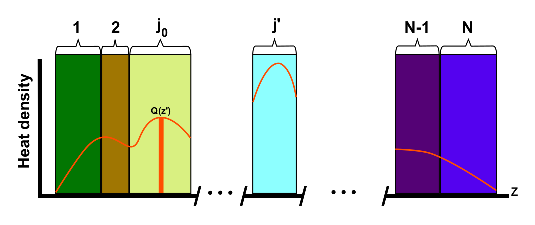
\includegraphics[width=0.4\textwidth]{General_plots_3.eps}
	\caption{Discretized stack of multiple layers for solving the 1D heat equation. The line indicates the heat density distribution $H(z)$. Top labels enumerate individual slices in the stack, each of which has its own thermal conductivity $\kappa_{j'}$ and thickness $L_{j'}$. }
	\label{fig:MultiLayersSetup}
\end{figure}
Note that Eq.~(\ref{eq:1Dheatequation}) can be solved in terms of discretized slices being considerably thinner than the actual layers. However, such a refined discretization is usually necessary only if the heat generation profile is non-uniform.
The full expressions for the solution $T(z)$ are given in the Supporting Information. 

With the general steady-state solution at hand, we can construct the effective heat transfer coefficients $h_{L}$ and $h_{R}$ that represent the thermal transport behavior of all layers between the ambient environment and the electrical contacts. $h_{L}$ and $h_{R}$ will serve as boundary conditions for the heat equation that is solved in the region between the contacts.
Since we presume that the heat is exclusively generated in the region between the contacts and that this heat flows out of the device, we can interpret $h_{L/R}^{-1}$ as the total thermal resistance due to all layers the thermal flux had to pass through on its way to respective edge of the device.
Such substrate- or encapsulation-sided thermal resistances consist of the sum of all individual thermal resistances that are located between the contact and the ambient environment, be them due to (i) the heat transfer coefficient $h_{i,j}^{-1}$ at each interface between layers $i$ and $j$ or due to (ii) the thermal conductivities ${L_i}/{\kappa_i}$ in each layer $i$.  
Recalling that $h_{E/S}^{ext}$ is the thermal transport coefficient of the interface between the outermost encapsulation (/substrate) surface and the ambient environment, we get:
\begin{equation}
\frac{1}{h_{L/R}} = \frac{1}{h_{E/S}^{ext}} + \sum \frac{L_i}{\kappa_i}.
\label{eq:effectiveh}
\end{equation}

\subsection{Device layout}
A major challenge for the simulation of the transport through the layers and across the layer interfaces is the large number of required parameters.
Each layer requires the heat conductivity $\kappa$ and a set of parameters that describe charge transport. 
Each pair of interfaces requires parameterized conditions that ensure charge and energy conservation, such as heat transfer coefficients and injection currents. 
An unbiased systematic variation of all these parameters yields only limited insight and does not provide leads for relevant relations without generating a very large set of data.
Therefore, we seek a model device for our simulations, that serves three purposes: 
(i) The device layout should support the setup of a toy model with which the role of the heat transfer coefficients $h$ towards the environment and the heat conductivities $\kappa$ of the organic layers can be conveniently distinguished.
(ii) The toy model should operate with a strongly reduced amount of parameters so that the impact of charge and heat transport can be disentangled best.
%(iii) The methodology chosen to treat the toy model must straight-forwardly accommodate more involved device structures.
(iii) It must be possible to straight-forwardly extent our toy model to accommodate more involved device structures with our modeling methodology.

Figure~\ref{fig:setup}-a shows a cross-section of a suitable device. 
While state-of-the-art devices contain a large number of distinct layers, we explicitly consider here two organic layers in which either predominantly hole or electron transport takes place. 
The two organic semiconducting layers are sandwiched between an anode and a cathode.
The organic layer adjacent to the cathode assumes the role of a electron transport layer while the one adjacent to the anode preferentially transports holes.
The division into two organic layers that form a heterojunction allows us to account for multiple conceivable charge transport scenarios in an effective manner.
Elaborate stacks for encapsulation or substrates are accounted for in this cross-section by one substrate and one encapsulation layer to capture their characteristic thickness and thermal properties. In general, however, the thermal behavior of the full sub-stacks that are not electrically active can be cast into effective heat transfer coefficients.
 
In a next step, we construct the device to be symmetric from a thermal point of view, because this symmetry halves the amount of free parameters necessary to describe thermal and charge transport. 
%As there is no differentiation between top (encapsulation) and bottom (substrate) anymore, i.e., no distinction between $h_L$ and $h_R$, we can consider only one parameter $h$.
As there is no differentiation between top (encapsulation) and bottom (substrate) anymore, we can use a common effective heat transfer coefficient $h$ rather than distinguishing between $h_L$ and $h_R$.
%we can more clearly track the impact of $\kappa$ and $h$. 
To guarantee the desired symmetric distribution of the heat density, two conditions must be fulfilled.
Firstly, the layers left and right of the device center must have equal thermal conductivities $\kappa$.
With having reduced our thermal parameters to $\kappa$ and $h$, we can more clearly track their impact on the device temperature and performance.
%and (ii) contribute equally to the electric current density.
Secondly, also the electric current density responsible for heat generation must be equal in the layers left and right of the device center.
This condition of balanced current halves the amount of necessary electrical parameters.
%A symmetric distribution of generated heat density is formed in the device if the layers left and right of the device center contribute equally to the electric current density and have equal thermal conductivities $\kappa$. We constructed such a symmetric device by placing the organic-organic junction in the center, i.e., assuming equal layer thicknesses, and adjusting the charge transport parameters in each layer to obtain equal current densities. Note that this adjustment condition allows us to impose mostly realistic charge transport parameters.  
% do not understand this argument
%This is not too crude approximation for organic layers, because their mobilities in general can vary a lot \cite{Blakesley2014}.
If realistic parameters are imposed for one layer, only parameters of the second layer require an adjustment to balance the current. 
In practice, the adjusted parameters are either the electron or the hole mobility in their respective transport layer or the offset between either the electron or the hole transport levels. 
A prototypical symmetric heating profile is shown in Figure~\ref{fig:setup}-b. We propose that such symmetric devices are ideal starting points to monitor the impact of subtle changes in the coupling between charge and heat transport.

%While in symmetric situation one can be sure about precise location of maximum temperature, we can not tell the same already in the 2-layers situation. Therefore, in general case, to obtain maximum temperature one should first calculate total temperature profile and then look for the maximum.
% \begin{subequations}
% 	 \begin{align}
%       T_k^L(x) = \frac{Q w C_R}{C_L + C_R} \left(\sum_{i=1}^{k-1} \frac{L_i}{\kappa_i} + \frac{1}{h_L} + \frac{x}{\kappa_k} \right) \\
%       T_k^R(x) = \frac{Q w C_L}{C_L + C_R} \left(\sum_{i=k+1}^{N} \frac{L_i}{\kappa_i} + \frac{1}{h_R} + \frac{L_k-x}{\kappa_k} \right) \\
%       T_k^H(x) = - \frac{Q(x-t)^2}{2 \kappa_k} +  \frac{Qw C_R}{\kappa_k (C_L+C_R)} (x-t) + \frac{Qw C_R}{C_L+C_R} \left(C_L- \frac{w}{2\kappa} \right) \\
%       C_L = \left( \frac{1}{h_L} + \sum_{i=1}^{j-1} \frac{L_i}{\kappa_i}+\frac{t+\frac{w}{2}}{\kappa_j} \right) \\
%       C_R = \left( \frac{1}{h_R} + \sum_{i=j+1}^{N} \frac{L_i}{\kappa_i}+\frac{L_j-t-\frac{w}{2}}{\kappa_j} \right)
% 	\end{align}
% \end{subequations}

\subsection{Material and geometry parameters.}
If not otherwise specified, we use the following parameters to setup our symmetric model OLED.
Each organic layer in our symmetric model device is 50~nm thick. 
The parameters for the electron transporting layer are inspired by Alq$_3$ and for the hole transporting layer by $\alpha$-NPB.
The offset between the electron transport levels is 0.3~eV, the offset between the hole transport level is the same. 
In each layer, the charge that is preferentially transported is considered with a charge carrier mobility $\mu_{high}$, whereas the charge of opposite polarity is considered with $\mu_{low}$. 
The mobilities are $\mu_{high}~=~6~\cdot~10^{-9}$ and $\mu_{low}~=~6~\cdot~10^{-10}$~\mobility, regardless whether electrons or holes are concerned. 
In the simulation, these mobility values correspond to the limit that the mobility attains for low electric fields and low charge carrier densities at room temperature. 
The relative dielectric permittivity $\epsilon_r$~=~3.5.
We disregard a direct thermoelectric coupling in our simulations by setting the Seebeck coefficient $S$ to zero.
Considering the typical values of $S~=~500~\mathrm{\mu V~K^{-1}}$ in organic semiconductors, the related thermal voltages $S \mathrm{\nabla} T$ are small compared to the applied voltage.
With this premise, the Seebeck coefficient has a negligible effect on the temperature and charge distribution and its disregard speeds up the simulations. 
%
We are using for both organic layers a mass density $\rho~=~2490~\mathrm{kg~m^{-3}}$ and a heat capacity $c_p~=~800~\mathrm{J~K^{-1}}$.
Note that mass density and heat capacity will not affect the steady state according to Eq.~(\ref{eq:contT}); rather, they affect the time scale in which steady state is reached.
Thermal conductivities of the organic layers realistically vary\cite{Reisdorffer2014} between $0.1~<~\kappa~<~1$~\thermalconductivity. They are inferior to the thermal conductivity  $0.8~<~\kappa~<~1$~\thermalconductivity~of ordinary glass,  ($\kappa$~=~1.022~\thermalconductivity~for a glass cover).

%-------------------- RESULTS -----------------------------------------------------------------------------------------------------------------------
%\section{Impact of $\kappa$ and $h$ on the OLED operation}
\section{Impact of thermal properties on the OLED operation}

\begin{figure}
	\centering
    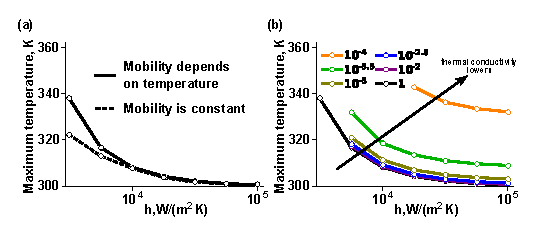
\includegraphics{Fig_3.eps} 
    \caption{(a) Difference between taking into account mobility dependence on temperature and having constant mobility. (b) Dependence of maximum temperature in the device on the thermal transfer coefficient $h$ for different heat conductivities (given in \thermalconductivity) for the device shown in Figure \ref{fig:setup} operated at 5~V. 
    For low values of $h$, particularly in combination with $\kappa$ values exceeding $10^{-3.5}$~\thermalconductivity~, such maximum temperatures cannot be given, because the generated heat cannot be fully dissipated from the device into its environment. Hence, the device heating never stops and the simulations fail to converge.}
\label{fig:I-Vandh-k-maxT}
\end{figure}

\subsection{Contributions to heating}
As a starting point, we explore how the generated heat is distributed across our symmetric model OLED operated at $V$~=~5V and at room temperature $T_{\mathrm{ambient}}$~=~300~K. 
Characteristic heat density distributions for three different values of $\kappa$ = $10^{-2}$, $10^{-3}$, and $10^{-4}$~\thermalconductivity %~and $h$~=~$10^{4.25}$~\hcoefficient 
are shown in Fig. \ref{fig:setup}-b.
Regardless of the values of $\kappa$ and $h$, these distributions are inherently symmetric with respect to the device center and consist of two distinct contributions. 
(i) The heat density features a sharp peak at the center. 
This contribution arises from the non-radiative electron-hole recombination that is localized at the organic-organic heterojunction. 
(ii) Joule heating is caused by the flow of charge carriers and stretches essentially throughout the entire cross-section. 
The largest amount of Joule heat is produced in the center, where the electric field that drives the current is highest. 
Correspondingly, the heat density drops from the center towards the contacts. 

The temperature distribution across the OLED is shown in Fig.~\ref{fig:setup}-c. Inherent to the symmetric profile of the generated heat, the temperature attains its maximum in the device center at the heterojunction. This maximum temperature depends on the value $\kappa$. However, only for a $\kappa$ as low as 10$^{-4}$~\thermalconductivity a maximum temperature is established that significantly exceeds the ambient temperature (by 40~K).   

\subsection{Heat transfer coefficient vs. thermal conductivity}
To systematically clarify, how the temperature distribution $T(z)$ changes with $h$ and $\kappa$ for a given voltage, we performed simulations in which the values of the thermal conductivities and heat transport coefficients varied by several orders of magnitude. 
To learn which combinations of $\kappa$ and $h$ lead to realistic and significant temperature elevations (from 1 to 100~K above room temperature), we intentionally also incorporated values for $\kappa$ and $h$ that materials cannot necessarily attain.
The maximum temperature taken from the simulated temperature distributions is shown as a function of $h$ for several values of $\kappa$ in Figure \ref{fig:I-Vandh-k-maxT}-b. 
Elevated maximum temperatures occur if either $h$ or $\kappa$ are small. Small values of $h$ and $\kappa$ correspond to a situation, in which we reduce the ability to dissipate heat from the OLED and, hence, store more heat inside.
The thermal conductivities of the organic layers in the OLEDs, expected to be between 0.1 and 1 \thermalconductivity, have a negligible impact on the temperature; the associated temperatures in Figure~\ref{fig:I-Vandh-k-maxT} are indistinguishable.
Even when taking a seriously underestimated thermal conductivity of 0.01 W/mK, the corresponding temperature distribution in Fig.~\ref{fig:setup}-b (red line) exceeds the ambient temperature by less than 4~K. 
This rather unexpected, negligible impact of $\kappa$ roots in the fact that the typical thickness of the electrically active layers is not large enough to sustain a temperature gradient inside the layer. To see this, we develop the following rationale: 

For our device consisting of two electrically active organic layers, we determine the highest, $T_{\mathrm{max}}$, and the lowest temperature, $T_{\mathrm{min}}$, inside the OLED with the help of the steady state heat flow equation (Eq.~(\ref{eq:1Dheatequation})) for given operating conditions. These solutions $T_{\mathrm{max}}$ and $T_{\mathrm{min}}$ are then interpreted in terms of $\kappa$ and $h$.
The maximum temperature $T_{\mathrm{max}}$ serves us as an indicator, how well the materials and operating conditions support the heat dissipation from the device. 
Combining $T_{\mathrm{max}}$ with $T_{\mathrm{min}}$, we also get largest temperature difference with the device.
To ease a subsequent interpretation, we approximate the heat density distribution $H(z)$ with a centered uniform profile $H_{\mathrm{uni}} = const$. 
Choosing the extension of the uniformly heated region to be $2x$ (cf. Fig.~\ref{fig:setup}-b), the totally heat generated with this profile is $2 x H_{\mathrm{uni}}$.
The lowest temperature is adopted on the device surfaces, $T_{\mathrm{min}} = T(0) = T(L)$. 
Given the arc-like shape of the temperature distribution (cf. Fig.~\ref{fig:setup}-c), that is symmetric for our model devices, $T_{\mathrm{max}}$ is located in the center of the device $T_{\mathrm{max}}$~=~$T(L/2)$.
%
Hence, we get $T_{\mathrm{max}}$ and $T_{\mathrm{min}}$  from the general solution $T(z)$ of the steady state heat flow equation Eq.~(\ref{eq:1Dheatequation}) (cf. Supporting Information for full expression) at $z~=~0$ and $z~=~L/2$, respectively:
\begin{subequations}
      \begin{align}
      	T_{min}=&\, x H_{\mathrm{uni}}\, \frac{1}{h},                                             \label{eq:analtmin}\\
        T_{max}=&\, x H_{\mathrm{uni}}\, \left(\frac{1}{h}+\frac{L - x}{2\kappa}\right) .		 \label{eq:analtmax}
      \end{align}
      \label{eq:analt} 
\end{subequations}
%
Both temperatures are proportional to the total heat generated in the device, $2 x H_{uni}$.
The surface temperature $T_{min}$ is inversely proportional to $h$, but does not contain any dependence on the thermal conductivities of the electrically active layers.
The temperature $T_{max}$ is determined by two terms, one being inversely proportional to $h$ and one being inversely proportional to the thermal conductivity $\kappa$. 
This second term conveys two important insights:
Firstly, the thermal conductivity influences $T_{max}$ the lesser, the less concentrated the generated heat profile is, i.e., the smaller difference $L-x$ between thickness $L$ of the layers and the halfed extension $x$ of the heat density profile is.
Secondly, even in a best-case estimation, in which we insert realistic values $L$~=~150~nm and $\kappa$~=~0.1~\thermalconductivity, the $(L-x)/\kappa$ remains with $\leq$ 1.5~\thermalconductivity~at least an order of magnitude smaller than the 1/$h$ contribution.
The thermal conductivity of the organic materials would non-negligibly contribute to $T_{max}$ if the organic films were at least a factor of ten thicker.

At this point, the irrelevance of the thermal conductivity $\kappa$ for thermal transport in realistically thin organic films has two important consequences.
Firstly, the actual bottleneck for heat dissipation is the combined thermal transfer between the contacts and the exterior, i.e., the thermal conductivities of layers being not electrically active and the associated heat transfer coefficients.
Vice versa, the layers that are responsible for electric transport are not relevantly involved in heat dissipation. 
This implies that the thermal and electrical properties can be optimized \textit{independent} from each other in complementary regions of the device to reach a desired performance. 
%, 
Secondly, the temperature within the organic layers is uniform, i.e., $T(z)$ = $T$ = const.
Then, $T$ can be immediately related to the total amount of generated heat per unit area, $H_{tot}$, via the heat balance equation $h_L T + h_R T = H_{tot}$:
%
\begin{equation}
	T=\frac{H_{tot}}{h_L+h_R}.
    \label{eq:onlyh}
\end{equation}
%
Note we do not require a symmetric device to establish this relation. 
$H_{tot}$ equals $H_{uni}~x$ in the case of a rectangular heating profile.
The heat transfer from the contacts to their associated device surfaces is fully accounted for in the effective heat transfer coefficients $h_L$ and $h_R$.  




%In the I-V curves we have already seen that high cooling parameters were responsible for instability in term of voltage fluctuations, while here for low thermal transfer parameters heating we indicate another instability.


%As we already stated, these simulations were performed under certain circumstances, namely with fixed device thickness and electric properties. Therefore it will be beneficial to have more general way to obtain these results for different conditions. For that reason we propose an analytical solution to the 1D device model. \newline\newline



\subsection{Impact of heat transfer $h$ on the current-voltage characteristics}
%\begin{figure}
%\centering
%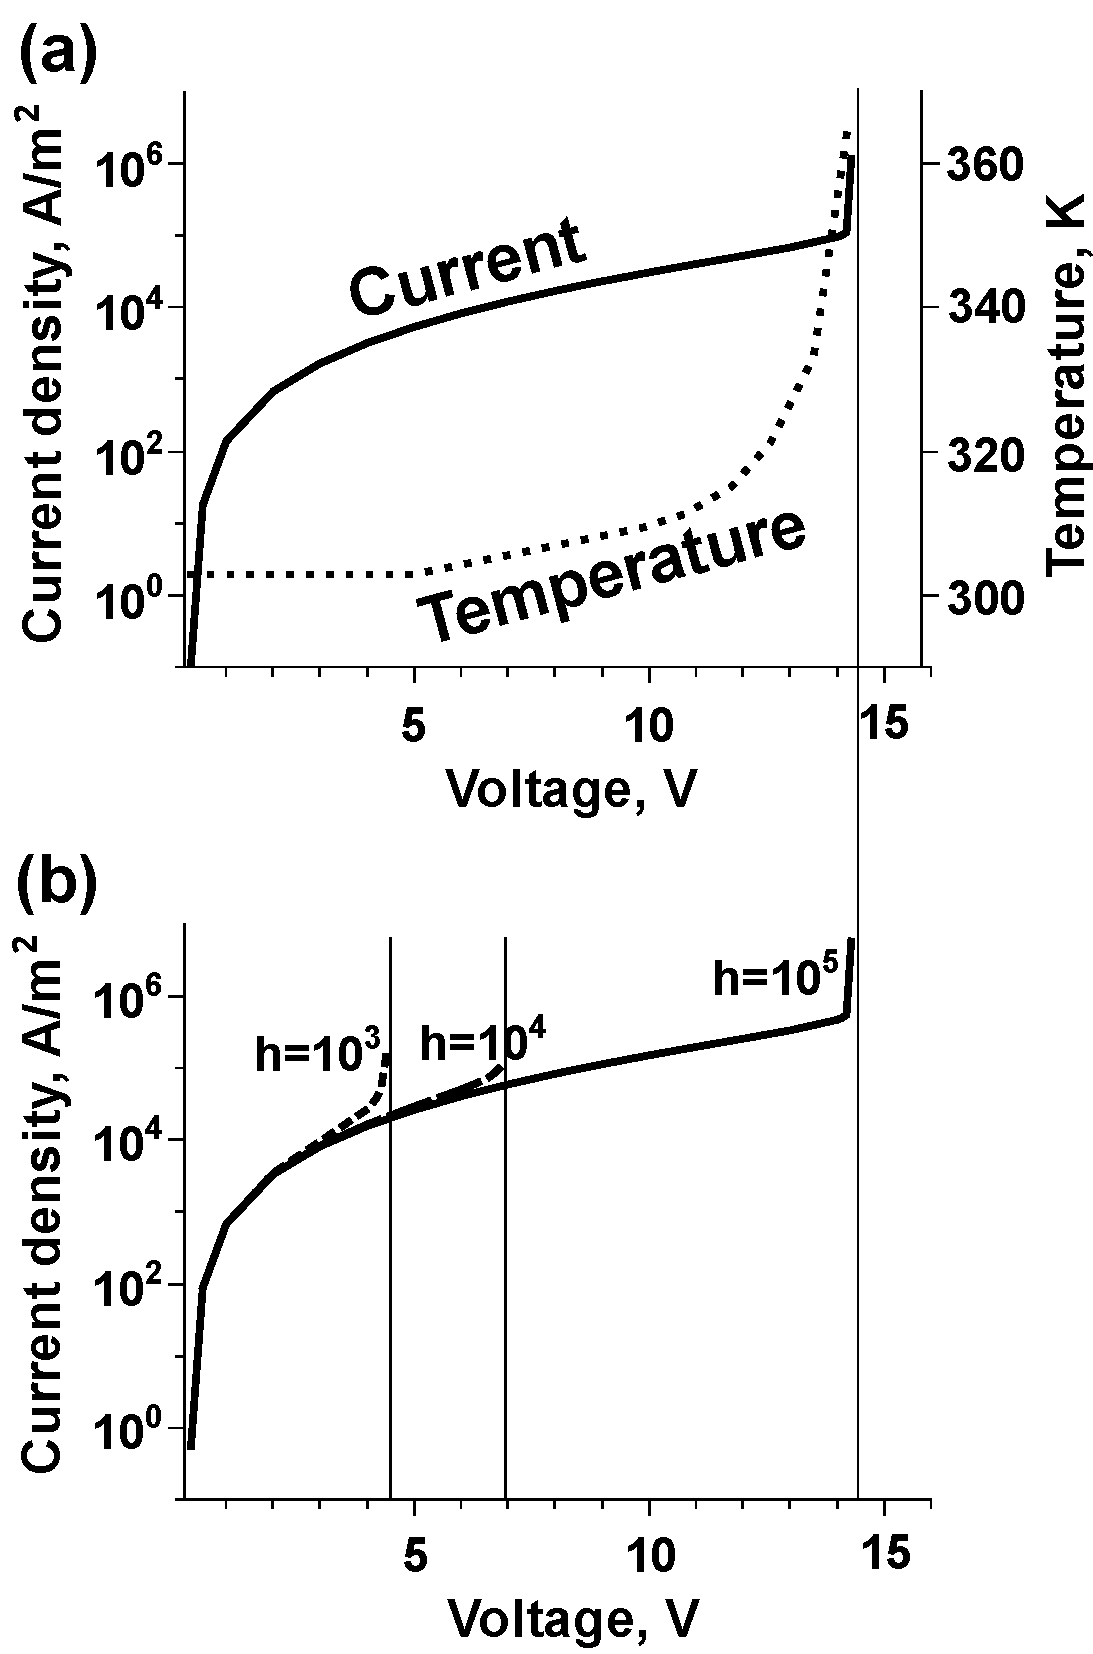
\includegraphics[width=0.5\textwidth]{I-V} \label{fig:I-V}
%\caption{Current-voltage characteristics under different heat transfer coefficients. All characteristics follow the same trend, but diverge at some point. This points determines voltage, where current is enough to put the device into vicious cycle. }
%\end{figure}
%With the nature of the heat density distribution established, the 
With having established that the thermal conductivity has a negligible impact on the device temperature, we turn to a closer inspection of the role of $h$.

If the maximum temperature is already markedly elevated, as seen in Figure \ref{fig:I-Vandh-k-maxT} for the smaller $h$, small changes in $h$ cause a large change in the temperature.
This finding is potentially relevant if one considers to operate the OLED considerably above room temperature, as such an elevated temperature promotes the electric conduction and radiative recombination. Subtle changes in the OLED layout, e.g., in terms of the thickness of the encapsulation layer, may strongly alter the temperature in the device, possibly even pushing the device in the regime of insufficient cooling and, concomitantly, into self-heating and thermal run-away.
%that the higher is the device temperature, the larger is the device response on $\kappa$ and $h$. 
%This is very important result - higher operating temperature for OLED devices can be preferable, because temperature inherently enhances electric properties and therefore should boost device effectiveness. 
%From this plot we can conclude - it is in general complicated to deduce optimal device operating conditions in terms of $\kappa$ and $h$, because of the tradeoff between stability and efficiency. 


%In the previous section we have shown that thermal conductivity has no impact on device temperature, while the device was under bias of 5V. Doubtless, the bias on its own is also responsible for device heating. 
In a next step we explore how $h$ affects the electric current and heating for different applied voltages.
To obtain a current-voltage characteristic, we computed the current for each external voltage anew starting out from an operating temperature equal to the ambient temperature. Hence, the computed I-V curves correspond to electric measurements that allow the device to sufficiently cool between consecutive current acquisitions.

Figure~\ref{fig:I-V}-a shows the current of the symmetric model OLED with $\kappa$~=~1~\thermalconductivity~and $h$~=~10$^{5}$~\hcoefficient~operated at room temperature $T$~=~300~K a function of the applied voltage.
%
\begin{figure}
\centering
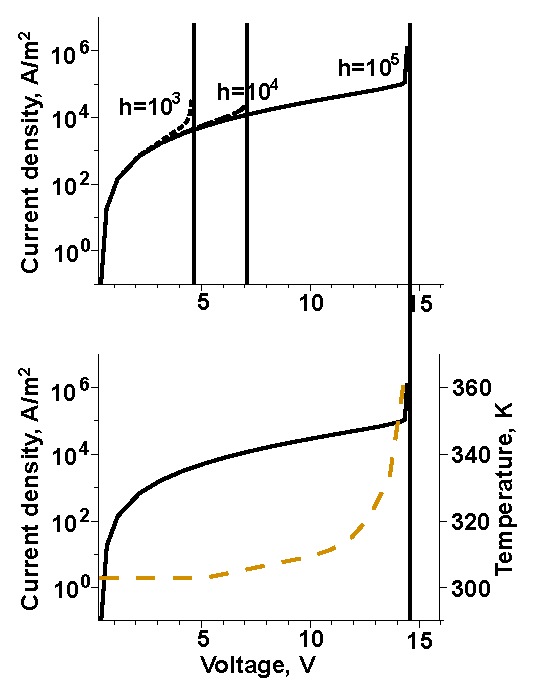
\includegraphics{I-V.eps} 
\caption{(a)~Current (solid line) and temperature (dashed line) against voltage for the device shown in Figure \ref{fig:setup} for $\kappa$~=~\thermalconductivity~and $h$~=~10$^{5}$~\hcoefficient~operated at room temperature $T$~=~300~K. The voltage at which the current diverges is indicated with a vertical line. Beyond this voltage, the temperature inside the device rises too quickly to allow a full heat dissipation and prevents a stable device operation (vicious cycle). (b)~Current-voltage characteristics for heat transfer coefficients $h$ between 10$^{3}$ and 10$^{5}$~\hcoefficient. The characteristics coinside at small voltages. The better the device is cooled (the larger $h$), the larger is the voltage, beyond which the current diverges (indicated by vertical lines).}
\label{fig:I-V}
\end{figure}
%
As the voltage is increased, the current and the temperature increase. 
Remarkably, also the thermal runaway process can be readily identified in this plot as an abrupt end of the recorded current-voltage curve that is preceeded by a sharp kink. The corresponding voltage is indicated by a vertical line in Figure~\ref{fig:I-V}-a.
Beyond this operating voltage, it is not possible to establish a stable current, because the heat is not sufficiently removed from the device anymore. The better the device is cooled, i.e., the larger the value of $h$, the larger is the critical voltage up to which the OLED operates. 

This impact of cooling is illustrated in Figure~\ref{fig:I-V}-b, that shows the evolution of the current density - voltage relation for the same charge transport parameters upon increasing the heat transfer coefficient $h$ from $10^3$ to $10^5$ \hcoefficient. 
The former value corresponds to the least efficient and the latter value to the most efficient cooling.
Again, the operating voltage in which we find the maximum current density and beyond which the current fails to converge is marked with a vertical line. 
All three current voltage characteristics coincide as long as the OLED is operated safely below 4.5~V.
%However, if one approaches the critical voltage, e.g., 4.5~V, there are pronounced differences in the current. 
%As the charge transport parameters are the same for all three current voltage characteristics, these curves coincide as long as they are operated safely below their critical voltage.
%
For the least efficient cooling considered, $h$~=~10$^3$~\hcoefficient, the current at 4~V is an order of magnitude larger than the current for a much more efficient cooling ($h \leq 10^4$ \thermalconductivity). Already small fluctuations in the operating voltage may cause a thermal runaway.
The current voltage characteristics do not only reflect the material and geometrical properties of the active layers, but also account for the properties of the exterior layers and, in effect, operating conditions, e.g., whether convective cooling applies.


\subsection{Extraction of heat transfer coefficients from experiment}

We have developed a rationale (Eq.~(\ref{eq:onlyh})), according to which the temperature $T$ in the electrically active layers is determined by the ratio between the total heat generated per unit area, $H_{tot}$, and the effective heat transfer coefficients $h_{(L/R)}$ between the electrically active region and the exterior with ambient temperature. 
With this relation at hand, the question arises whether it is possible to obtain the totally generated heat density $H_{tot}$ directly from experiment to get an estimate for either $h_L$ and $h_R$ for a known device temperature $T$ or $T$ for known $h_L$ and $h_R$.
Such an estimation is valid as long as the heat transported away from the electrically active region does not influence the temperature inside the this region and preserves a uniform temperature distribution. 

The total heat density $H_{tot}$ consists of the Joule heat $H_J$ and the heat $H_{\mathrm{rec}}$ due to non-radiative recombination.
Knowing the current voltage characteristics, $I(V)$, the Joule heat per unit area $S$, $H_{J}$, is readily given by
\begin{equation}
		H_{J}= \frac{I V}{S}. \label{eq:JouleHeating} 
\end{equation}
The recombination heat per unit area $S$, $H_{\mathrm{rec}}$, equals
\begin{equation}
		H_{\mathrm{rec}} = \frac{(1-\eta_\mathrm{i}) I E_R(eV)}{S}. 		\label{eq:RecombinationHeating}
\end{equation}
Therein, the coefficient $1-\eta_i$ ensures that exclusively triplet exciton states are considered for the heating and $E_R(eV)$ is the recombination energy, measured in electron-volts. 

Inserting Eqs.~(\ref{eq:JouleHeating},\ref{eq:RecombinationHeating}) into the analytic equation Eq.~(\ref{eq:analtmax}) for the maximum temperature, we arrive at:
\begin{equation}
	T_{\mathrm{max}}=\frac{ V+(1-\eta_i) E_R\left(eV\right) }{h_L+h_R} \frac{I}{S}.
    \label{eq:TmaxAsAFunctionOfIVErec}
\end{equation}


We subjected this relation for $T_{\mathrm{max}}$ to a consistency check to reveal whether we can safely exclude a possible feedback from the heat transported through the encapsulation and substrate layers on the temperature inside the electrically active layers.
To this aim, we compared the value $T_{\mathrm{max}}$ extracted from the full simulation with the value obtained from Eq.~(\ref{eq:TmaxAsAFunctionOfIVErec}), in which we inserted only the current densities obtained from  the simulations. For a realistic thermal conductivity of 0.5~\thermalconductivity~with an voltage of 5 V applied, we calculated maximum temperature from Eq.~(\ref{eq:TmaxAsAFunctionOfIVErec}). 
Eq.~(\ref{eq:TmaxAsAFunctionOfIVErec}) reproduces the exact temperature values for a large range of heat transfer coefficients $h$; for $h_L + h_R \geq 10^{4}$~\hcoefficient~the relative error in predicted temperatures remains below 1~\%. 
Only when $h$ approaches values for which the device starts to overheat, either a deviation ($4\cdot 10^3 \leq h_L + h_R \leq 10^4$ \hcoefficient) or thermal runaways are obtained ($h_L + h_R \geq 4\cdot 10^3$ \hcoefficient). 
Details are shown in the Supporting Information.

\section{Conclusions}

We investigated how the thermal conductivities of the electrically active organic layers and the heat transfer between the electrically active region and the ambient environment determine the temperature distribution inside OLEDs under operating conditions.
To this aim, we established a macroscopic, three-dimensional drift-diffusion based simulation that incorporates charge transport, thermal transport and their mutual coupling for a given OLED stack.
In particular, we account for the feedback mechanism of self-heating, that occurs when any dissipation of heat within electrically active layers boosts their electric conductivity which, in turn, enhances the generation of heat.
This model allows us to monitor the time-dependent and steady-state behavior of the temperature, the charge carrier densities, the current densities, and local electric fields.

%A steady state is reached only, if the heat is sufficiently well removed from the device to counter-balance self-heating.
The OLED reaches steady state operation only if the heat is sufficiently well removed from the device to counter-balance self-heating. 
If either the thermal conductivities or the heat transfer coefficients fall below a certain limit, a blocked outflow of heat and self-heating promote a steep increase in the temperature inside the OLED with rising applied voltage. 
For such a choice of the thermal parameters, any other change in the OLED setup or any fluctuations in operating conditions can trigger the thermal runaway process.

% First of all, when one decreases any transport parameter beyond some limit, temperature rapidly ramps up. Moreover, because heat transport is coupled to electric transport, this increase comes not only from blocked heat outflow, but also because the device heating itself increases. From more practical point of view it means that the device can operate in 2 regimes. When the temperature compared to ambient temperature is low (by "low" we mean at maximum several degrees), OLED is not sensitive to the thermal transport parameters changes and we assume that it will be more stable under structural changes, which are part of OLED's degradation. When the temperature increases above that, device becomes unstable and any fluctuations in operating conditions can start runaway process.

The thermal conductivity of realistically thin organic layers only marginally affect the temperature in the device; in fact, the temperature adopted in an electrically active organic layer is essentially constant. 
The temperature profile across the entire stack is determined by the thermal properties of the encapsulation layers, the substrate layers, and the heat transfer coefficient associated to heat exchange between the outermost OLED surfaces and the ambient environment.
Self-heating arising from an inadequate heat dissipation from the heat source towards the exterior, e.g., due to a limited choice in terms of the substrate, can neither be counter-balanced by a larger thermal conductivity, nor by thicker organic films. 
% Utilizing analytic solution on 1D heat equation, we show that temperature increase coming from h-coefficient and thermal conductivity comes separately and additively. 
% Therefore, if excess temperature came from one parameter, one cannot compensate it by tuning another one. Thus, existing device problems come from low h-coefficient, i.e. inefficient heat outflow and to beat them we should be more careful with the choice of the substrate. 

The layers responsible for the major electrical effects differ from the layers in which the relevant thermal effects occur, despite the fact that charge and heat transport strongly couple in the electrically active layers. 
From a practical point of view that means that the charge transport can be considered and optimized assuming a fixed temperature (e.g., in Kinetic Monte Carlo simulations). The temperature distribution across the entire stack can be, in turn, provided by solving the heat transport equation for the layers outside the electrically active substack.

% may influence real world device only in very low, unphysical range. This means that relatively high thermal conductivity we have in organic layers makes temperature profile almost flat across organic layers. This is important conclusion, because it essentially means that despite their strong coupling in the active layers, electric and thermal effects still can be attributed to different layers. From simulation/analytic point of view that means that it is enough to simulate organic layers under fixed temperature to get proper outcome (this is essentially always the assumption in Morte-Carlo studies of OLEDs), while heat equation should be solved outside the device to obtain temperature distribution. 

\section{Acknowledgement}
This work was funded by the Austrian Climate and Energy Fund (KLIEN) and the Austrian Research Promotion Agency (FFG) through the project “ThermOLED” [FFG No. 848905]. The authors would also like to acknowledge the use of HPC resources provided by the ZID of Graz University of Technology.


\clearpage
\bibliographystyle{aapmrev4-1} %aipnum4-1
\bibliography{New_citation.bib}
\clearpage

\section*{Supporting information.}

\subsection*{General analytic solution for the steady-state 1D heat equation}
% \begin{figure}
% 	\centering
% 	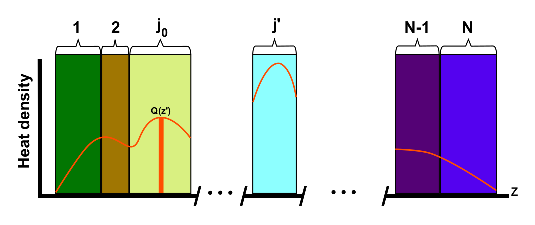
\includegraphics[width=0.4\textwidth]{General_plots_3}
% 	\caption{Discretization for solving the 1D heat equation for multiple layers. The orange line indicates the heat density distribution $Q(z)$. The top labels enumerate the layers, each of which has its own thermal conductivity $\kappa_{j'}$ and thickness $L_{j'}$. }
% 	\label{fig:MultiLayersSetup}
% \end{figure}


Utilizing a thermal conductivity function, in which a thermal conductivity $\kappa_j$ is assigned to each layer $j$ located along the $z$-axis (cf. Fig.~\ref{fig:MultiLayersSetup}), we can formulate a heat equation for the whole device.
The general solution of the differential equation (\ref{eq:1Dheatequation}) is given by a Green function $G(z,z_0)$ that solves Eq.~(\ref{eq:GreenFunctionEquation}). 

\begin{equation}
	-\left( \kappa(z) G_z'(z,z_0)  \right)_z' = \delta(z-z_0)
    \label{eq:GreenFunctionEquation}
\end{equation}

If one multiplies Eq.~(\ref{eq:GreenFunctionEquation}) by $H(z_0)$ and integrates it with respect to $z_0$, one obtains the following equation: %. 
\begin{equation}
	-{\left(\kappa (z) \left(\int_0^L dz_0 G(z,z_0) H(z_0) \right)_z' \right)}_z' = H(z).
	\label{eq:GreenFunctionHeatEquation}
\end{equation}

Therefore, the term in the inner bracket of Eq.~(\ref{eq:GreenFunctionHeatEquation}) should be equal to the $T(z)$ in the presence of the heat distributed as $H(z)$. 

If one returns to the equivalent notation with several layers and imposes the preservation of heat flux across the interfaces, one arrives at the equation: %.
\begin{equation}
	T(z) = \sum_{j'=1}^{N} \int_{z_{j'-1}}^{z_{j'}} H(z_0) G(z,z_0) dz_0.
    \label{eq:GreenFunctionSolution}
\end{equation}

Where $z_{j'}=\sum_{i=1}^{j'} L_i$ and $L_{i}$ refers to the thickness of the individual layers.
The Greens function $G(z,z_0)$ can then be conveniently written using functions $W^L(z)$ and $W^R(z)$ for each layer $b$:%in equations \ref{eq:greenfunction}.

% \begin{subequations}
% 	 \begin{align}
% 		W_b^L(z) =& \frac{1}{h_L}+\sum_{i=1}^{b-1} \frac{L_i}{\chi_i} + \frac{z}{\chi_b} \label{eq:WL}\\
%         W_b^R(z) =& \frac{1}{h_R}+\sum_{i=b+1}^{N} \frac{L_i}{\chi_i} + \frac{L_b - z}{\chi_b} \label{eq:WR}\\
%         G_{j,j'}^L =& \frac{1}{\sum_{i=1}^{N} \frac{L_i}{\chi_i}} W^L_{j}(z) W^R_{j'}(z'), z<z' \label{eq:GL}\\
%         G_{j,j'}^R =& \frac{1}{\sum_{i=1}^{N} \frac{L_i}{\chi_i}} W^R_{j}(z) W^L_{j'}(z'), z>z' \label{eq:GR}
% 	\end{align}
%     \label{eq:greenfunction}
% \end{subequations}

\begin{subequations}
	 \begin{align}
		W_b^L(z) =& \frac{1}{h_L}+\sum_{i=1}^{b-1} \frac{L_i}{\chi_i} + \frac{-\left( \sum_{i=1}^{b-1} L_i \right) + z}{\chi_b} \label{eq:WL}\\
        W_b^R(z) =& \frac{1}{h_R}+\sum_{i=b+1}^{N} \frac{L_i}{\chi_i} + \frac{\left( \sum_{i=1}^{b} L_i \right)  - z}{\chi_b}. \label{eq:WR}\\
	\end{align}
    \label{eq:Wfunction}
\end{subequations}

Then, the Green's functions $G^{L}(z,z_0)$ for $z<z_0$ and $G^{R}(z,z_0)$ for $z>z_0$ read:

\begin{subequations}
	 \begin{align}
        G_{j,j'}^L =& \frac{1}{\sum_{i=1}^{N} \frac{L_i}{\chi_i}} W^L_{j}(z) W^R_{j'}(z_0), \quad \mathrm{for~} z<z_0 \label{eq:GL}\\
        G_{j,j'}^R =& \frac{1}{\sum_{i=1}^{N} \frac{L_i}{\chi_i}} W^R_{j}(z) W^L_{j'}(z_0), \quad \mathrm{for~} z>z_0. \label{eq:GR}
	\end{align}
    \label{eq:greenfunction}
\end{subequations}

While $j$ and $z$ are the coordinates of the layer where one calculates temperature, $j'$ and $z_0$ correspond to that layer from which one want to calculate contribution to the temperature (cf.~Figure \ref{fig:MultiLayersSetup}). 
To obtain temperature distribution in certain layer $j$ at point $z$ for given heat distribution $H(z_0)$ according to Eq.~(\ref{eq:GreenFunctionSolution}), one should integrate $H(z_0)$ weighted with the corresponding Green function $G_{j,j'}(z,z_0)$ with respect to $z_0$ and sum the contributions from all layers $j'$ . 

\subsection*{Testing the consistency of the analytical model with simulation results.}

The maximum temperature predicted by the simplified Eq.~(\ref{eq:TmaxAsAFunctionOfIVErec}) corresponds well to the prediction of the full simulation for a large range of heat transfer coefficients.
Figure~\ref{fig:connection_to_experiment} shows the relative error,
$\frac{|T_{max,an} - T_{max,sim}| }{T_{max,sim}-300K} - 1$, between $T_{max}$ either predicted on the basis of Eq.(\ref{eq:TmaxAsAFunctionOfIVErec}) and the current obtained from the simulation ($T_{max,an}$) and $T_{max}$ directly obtained from the simulations ($T_{max,sim}$).

%----------------------------
% push into SUI
\begin{figure}[h]
	\centering
    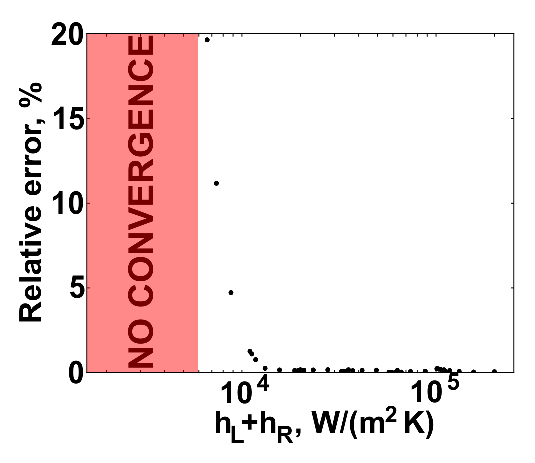
\includegraphics{General_plots_2.eps}
    \caption{Validity of the maximum temperature predicted by Eq.(\ref{eq:TmaxAsAFunctionOfIVErec}) as a function of the total heat transfer coefficient $h_L + h_R$. Shown is the relative error $\frac{|T_{max,an} - T_{max,sim}| }{T_{max,sim}-300K} - 1$ formed between $T_{max,sim}$ deduced from the full simulation and $T_{max,an}$ predicted from Eq.(\ref{eq:TmaxAsAFunctionOfIVErec}) using only the current obtained from the simulation. In the red shaded region, located at small $h_L + h_R$, the device overheats so that the simulations do not converge.}
    \label{fig:connection_to_experiment}
\end{figure}
%----------------------------------------

For $h_L + h_R < 4\cdot10^3$~\hcoefficient~, $T_{max,sim}$ cannot be determined, because thermal runaway prevents the convergence to a steady state (red shading).
Solely closely above the thermal runaway region, $h_L + h_R < 10^4$~\hcoefficient~, the temperature predicted by Eq.(\ref{eq:TmaxAsAFunctionOfIVErec}) deviates from the simulation. The prediction of Eq.(\ref{eq:TmaxAsAFunctionOfIVErec}) fails for these heat transfer coefficients, because the temperature distribution in the device is not uniform.

%It can be successfully used to determine how much the device will heat up under particular electric current and all other terms in this equation are accessible through experiment. 


\subsection*{Feedback between heat transport and device temperature.}

Here we intend to identify for which $h$ and $\kappa$ it is safe to assume that the heat transport away from the electrically active region does not affect the temperature of this region. 
For situations in which this assumption is invalid, we want to gather the symptoms of the electro-thermal feedback.
We check for the presence of an electro-thermal feedback by comparing the temperature distribution $T_{sim}(z)$ from the full simulation and $T_{an}(z)$ from solving the steady state heat transport equation, Eq.~(\ref{eq:1Dheatequation}).
Eq.~(\ref{eq:1Dheatequation}) is inherently unable to account for a possible feedback of the heat transport on the charge transport and the heat generation profile.
Hence, we can interpret any deviation of $T_{an}(z)$ from $T_{sim}(z)$ as a manifestation of a feedback.

Such a comparison is particularly feasible for our symmetric model OLED.
As the temperature distribution is symmetric, the largest temperature $T_{max}$ is always established in the device center (cf. Fig.~\ref{fig:setup}-c). Rather than accounting for the entire profiles $T(z)$,
it is sufficient to compare the predicted maxima $T_{max,an}$ and $T_{max,sim}$.
%Such a comparison is particularly feasible for our symmetric model OLED.
%As the temperature distribution is symmetric and the largest temperature $T_{max}$ is always established in the device center (cf. Fig.~\ref{fig:setup}-c), it is sufficient to compare the predicted $T_{max,an}$ and $T_{max,sim}$.
For sufficiently large $\kappa$ and $h$, we expect that the heat flow is large enough to prevent any heat accumulation in the electrically active region. 
Hence, the heat density profile $H(z)$ is independent of $\kappa$ and $h$. %and is solely governed by the electric properties and operating conditions.
Guided by Fig.~\ref{fig:I-Vandh-k-maxT}-b, we encounter this situation for $\kappa = 1$~\thermalconductivity~ and $h = 10^5$~\hcoefficient~ at an operating voltage of 5~V.  
The simulated heat density profile $H(z)$ retrieved for these thermal parameters gives rise to the total heat $H_{tot} = \int_0^L dz H(z)$. 
Since this $H(z)$ is solely governed by the electric properties and operating conditions, it will now serve as the input for Eq.~(\ref{eq:1Dheatequation}) to inspect $T_{an}$ for other values of $\kappa$ and $h$.

\begin{figure}
	\centering
	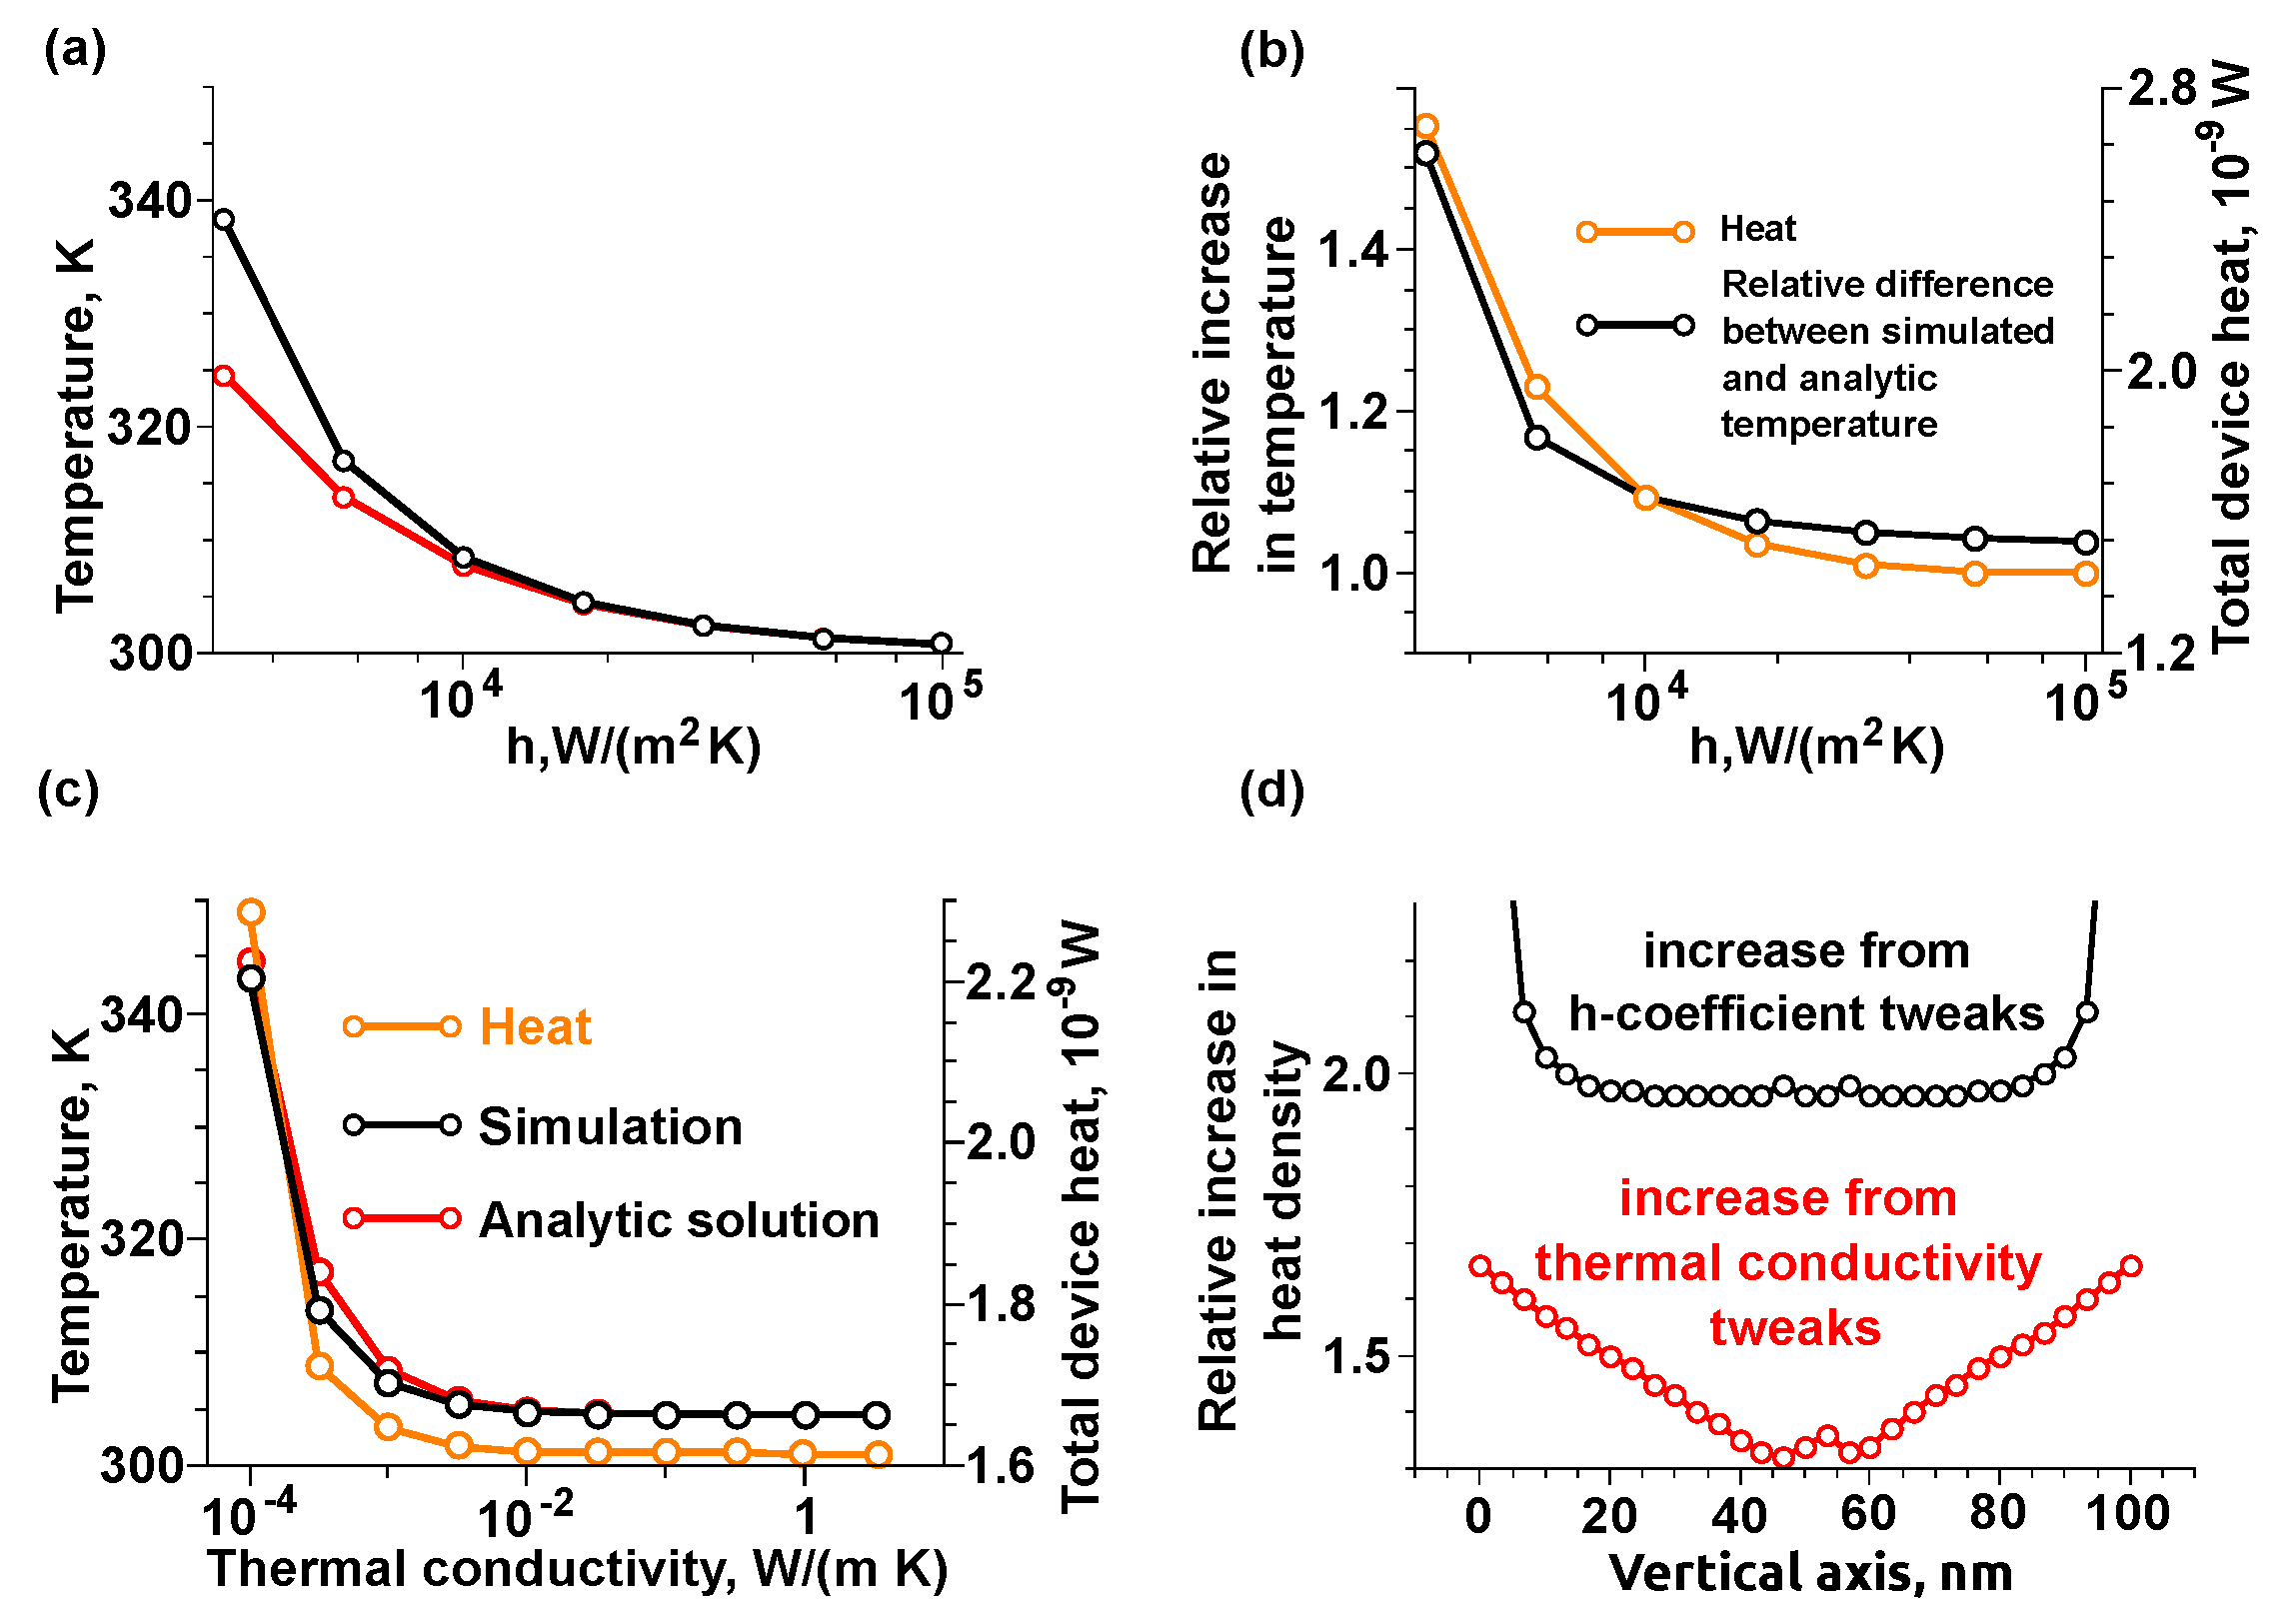
\includegraphics[width=0.75\textwidth]{General_plots_5.pdf}
	\caption{(a) Maximum temperature $T_{max,sim}$ (black) and $T_{max,an}$ (red) in the device as a function of the heat transfer coefficient $h$ at $\kappa$=1~\thermalconductivity. $T_{max,sim}$ are temperature values extracted from simulations of the model OLED operated at 5~V. $T_{max,an}$ are temperature values calculated from the analytical solution of Eq.~(\ref{eq:1Dheatequation}) using the heat generation profile obtained for $h=10^5$~\hcoefficient. (b) Relative increase in temperature, $\frac{T_{max,sim}}{T_{max,an}}-1$, (left axis) compared to the total device heat $H_{tot}$ (right axis) as a function of the h-coefficient. (c) Maximum temperature $T_{max,sim}$ (black) and $T_{max,an}$ (red) in the device (left axis) and $H_{tot}$ (right axis) as a function of thermal conductivity at h = $10^{4.25}$~\hcoefficient. (d) Local changes in heat density due a change in a thermal parameter. $\frac{H_{h}(z)}{H_{h_{ref}}(z)}-1$ monitors the relative change in heating density when going from $h = 10^{3.5}$ to $10^5$~\hcoefficient at $\kappa$ = 1~\thermalconductivity (black curve) and $\frac{H_{\kappa}(z)}{H_{\kappa_{ref}}(z)}-1$ the relative change in heat density in going from
	$\kappa = 1$ to $10^{-4}$~\thermalconductivity~for $h$ = $10^{4.25}$~\hcoefficient (red curve).}
	\label{fig:final4plots}
\end{figure}

Figure~\ref{fig:final4plots}-a shows the evolution of $T_{max,an}$ and $T_{max,sim}$ for varying heat transfer coefficients $h$ at $\kappa = 1$~\thermalconductivity. 
As long as $T_{max}$ remains smaller than 310~K, $T_{max,an}$ (red) and $T_{max,sim}$ (black) are indistinguishable.
Below $h \approx 10^4$~\hcoefficient, the simulations reveal a markedly larger temperature as one would expect from the analytical solution $T_{max,an}$. 
Not only the two temperatures $T_{max,sim}$ and $T_{max,an}$, but also the trend in the deviation between the two temperatures, cast for convenience into the expression $\frac{T_{max,sim}}{T_{max,an}}-1$ in Fig.~\ref{fig:final4plots}-b, is directly related to the total amount of heat $H_{tot}$ (orange) produced in the device.
Hence, the elevated temperature $T_{max,sim}$ is the symptom for the electro-thermal feedback between the transported heat and the heat density profile that causes self-heating.

Note that the equality between $T_{max,sim}$ and $T_{max,an}$ does not necessarily imply the absence of electro-thermal feedback. 
To illustrate that, Fig.~\ref{fig:final4plots}-c shows $T_{max,sim}$ and $T_{max,an}$ as a function of $\kappa$ at constant $h = 10^{4.25}$~\hcoefficient. 
At the first glance, $T_{max,sim}$ and $T_{max,an}$ coincide even for lowest probed $\kappa = 10^4$~\thermalconductivity.
%the heat transfer equation appears to correctly predict the maximum temperature in the OLED even for very low $\kappa = 10^4$~\thermalconductivity.
However, a closer inspection of the situation at such low $\kappa$ reveals that there is nevertheless an electro-thermal feedback and, hence, heat accumulation inside the electrically active layers.
This accumulation of heat predominantly changes the \textit{shape} of the heat density profile $H(z)$.
%To visualize this change shape, we plot the relative change of heat density, $\frac{H_{\kappa}(z)}{H_{\kappa_{ref}}(z)}-1$ (red curve), that occurs upon going from $\kappa$ = 1 (reference) to $10^{-4}$~\thermalconductivity, as a function of the position $z$ in the electrically active region in Fig.~\ref{fig:final4plots}-d.
To visualize how the heat density $H(z)$ differs in each position $z$ in the electrically active region between $10^{-4}$~\thermalconductivity and $\kappa$ = 1~\thermalconductivity, we plot the corresponding relative change of heat density, $\frac{H_{\kappa}(z)}{H_{\kappa_{ref}}(z)}-1$ (red curve) in Fig.~\ref{fig:final4plots}-d.
%While the heat produced at the organic-organic interface is not affected by $\kappa$.
%
%Lowering $\kappa$ leads to an enhanced heating closer to the surfaces. This additional heat diffuses more easily to the surfaces that to the center due to the non-uniform temperature distribution across the device. 
%This change in heat density does not occur uniformly across the device, but is rather V-shaped.
%Due to the arc-shaped temperature distribution across the OLED, the lowering of $\kappa$ causes the temperature to rise mainly in the center of the device and to a much lesser extent near the outer surfaces. 
This change in heat density does not occur uniformly across the active layers. 
Rather, regions are heated the stronger the closer they are to the surface.
Due to the arc-shaped temperature distribution across the within the active layers, a lowering of $\kappa$ causes the temperature to rise mainly in the center of the device and, to a much lesser extent, near the outer surfaces. 
While the temperate elevation increases the recombination and the electric conductivity at the device center, the electrical conductivity near the surfaces considerably lesser raised.
Since Joule heating is more pronounced in the regions with lower electrical conductivity, more heat is produced near the surface compared in the center.
%The correspondingly occurring V-shape  
%Temperature increases mainly in the middle of the device which in turn increases recombination and overall electric current. On the other hand, temperature close to surfaces is smaller and resistivity of layers is higher there. So, comparing heating in the center and close to surfaces, Joule heating is higher in the regions with low electrical conductivity. From the equation \ref{eq:analtmax} one can easily deduce that such changes in the shape affect maximum temperature and this is exactly what we see here.

For comparison, we also show that shape of the heat density profile $H(z)$ is essentially preserved when comparing excellent ($h$ = $10^{5}$~\hcoefficient) and inferior ($10^{3.5}$~\hcoefficient) heat transfer with the environment.
Fig.~\ref{fig:final4plots}-d (black curve) shows the corresponding relative change of heat density, $\frac{H_{h}(z)}{H_{h_{ref}}(z)}-1$.
Throughout the active layers, this change is practically uniform except for sudden increase in the close vicinity of the outer surfaces. The overall temperature profile is governed by these extended regions of uniform heating; the very narrow surface regions do not have a perceivable impact.


%Such enhanced heating contributions near the surface play a sub-ordinate role in establishing the temperature as these surface regions are small compared to the regions of uniform heating.

%Note that relative change appears to There are no real physical consequences for the device, because heating density in this region is small compared to other regions in the device and hard to notice absolute changes look substantial on relative scale. 
%We see that changing h-coefficient uniformly increases heating all across the device. 

%In this section we want to provide some overview how equations \ref{eq:analt} work in detail. We start investigation from taking a look on how heat transport coefficient affects temperature distribution. The whole system reacts to its change via complex mechanisms, therefore we are particularly interested when we can make simple conclusions from change in the device thermal structure and when they stop working. We start this investigation from fixing thermal conductivity and changing heat transport coefficient. This attempt is depicted in Figure \ref{fig:final4plots}-a. 

%\begin{figure}
%	\centering
%	\includegraphics[width=0.5\textwidth]{Graph2}
%	\caption{Maximum temperature in the device as a function of h-coefficient at point $\kappa$=1 W/(mK). Simulated temperatures are temperatures extracted from our simulations. Predicted temperatures are temperatures calculated from analytical model using first two points as reference ones.}
%	\label{fig:h-maxT-appmaxT}
%\end{figure}

%As one can see, reverse proportion rule of Eq. \ref{eq:analt} works until certain limit, roughly speaking, until around 310~K. After that, simulated temperature numbers diverge quickly from the predicted values. The difference of course comes from $H_{uni} x$ term, which corresponds to the total amount of heat generated in the device. The total generated heat as well as relative difference between two temperatures as a function of h are presented at Figure \ref{fig:final4plots}-b. 

%\begin{figure}
%	\centering
%	\includegraphics[width=0.5\textwidth]{Graph3}
%	\caption{Difference between relative temperature and total device heating.}
%	\label{fig:h-dT-H}
%\end{figure}

%From this one can easily see that most difference between equation \ref{eq:analtmax} and simulation comes from our ignorance about how the amount of generated heat depends on the change of h. We can see that when h-coefficient decreases, temperature rises by two mechanisms. First is the change of temperature due to less efficient heat outflow. But that temperature rise produces via electro-thermal coupling another effect of increased device heating. 

%With thermal conductivity the results are completely different, Figure \ref{fig:final4plots}-c. Suddenly, analytical model predicts the maximum temperature behavior very well in any region. Moreover, it even overestimates the result which was not the case with heat transport coefficient. The only way to understand it via analytic model is the second order term proportional to $x$ in the brackets. As the heating profile shrinks, it leads to the changes in temperature which are not governed by total heating. To look at that in more details we compared how heating profiles locally changes when we change separately heat transport coefficient and thermal conductivity. Results are presented at Figure \ref{fig:final4plots}-d

%\begin{figure}
%	\centering
%	\includegraphics[width=0.5\textwidth]{Graph5}
%	\caption{Maximum temperature in the device as a function of thermal conductivity at point h=17782 W/($m^2$K) (This corresponds to h=$10^{4.25}$). Simulated temperatures are temperatures extracted from our simulations. Predicted temperatures are temperatures calculated from analytical model using first two points as reference ones.}
%	\label{fig:k-maxT-appmaxT-H}
%\end{figure}

%So we see that the total device heating depends differently on thermal conductivity than on h-coefficient. The absolute values on this plot are not important, what we are looking for is the shape. Also, on the h-coefficient curve on can see that the edges are very much lifted up. There are no real physical consequences for the device, because heating density in this region is small compared to other regions in the device and hard to notice absolute changes look substantial on relative scale. 

%We see that changing h-coefficient uniformly increases heating all across the device. At the same time, changes of thermal conductivity lead to heating which is more profound close to the surfaces and therefore is easier to diffuse to the edge. This is the consequence of non-uniform temperature distribution across the device. Temperature increases mainly in the middle of the device which in turn increases recombination and overall electric current. On the other hand, temperature close to surfaces is smaller and resistivity of layers is higher there. So, comparing heating in the center and close to surfaces, Joule heating is higher in the regions with low electrical conductivity. From the equation \ref{eq:analtmax} one can easily deduce that such changes in the shape affect maximum temperature and this is exactly what we see here.

%\begin{figure}
%	\centering
%	\includegraphics[width=0.5\textwidth]{Graph7}
%	\caption{How local heating changes when one varies h-coefficient (black curve) or thermal conductivity (red curve). Black curve: $\kappa$ = 1 W/(mK), h-coefficient varies from $10^{3.5}$ to $10^5$ Red curve: h = $10^{4.25}$, $\kappa$ varies from $10^{-4}$ to 1. }
%	\label{fig:z-hdH-kdH}
%\end{figure}

% \begin{table}[]
% \makebox[\textwidth]{\begin{tabular}{|c|c|c|c|c|c|c|c|c|c|c|}
% \hline
% \diagbox{h}{$\kappa$}      & 0.0001 & 0.000316 & 0.001 & 0.00316 & 0.01  & 0.0316 & 0.1   & 0.316 & 1    & 3.16 \\\hline
% 1000   &\cellcolor{black!100}&\cellcolor{black!100}&\cellcolor{black!100}&\cellcolor{black!100}&\cellcolor{black!100}&\cellcolor{black!100}&\cellcolor{black!100}&\cellcolor{black!100}&\cellcolor{black!100}&\cellcolor{black!100}\\\hline
% 1780   &\cellcolor{black!100}&\cellcolor{black!100}&\cellcolor{black!100}&\cellcolor{black!100}&\cellcolor{black!100}&\cellcolor{black!100}&\cellcolor{black!100}&\cellcolor{black!100}&\cellcolor{black!100}&\cellcolor{black!100}\\\hline
% 3160   &\cellcolor{black!100}&\cellcolor{black!100}&\cellcolor{black!100}&\cellcolor{black!100}&\cellcolor{black!100}&\cellcolor{black!100}&\cellcolor{black!100}&\cellcolor{red!25}1.26&\cellcolor{red!25}1.26&\cellcolor{red!25}1.25\\\hline
% 5620   &\cellcolor{black!100}&\cellcolor{green!25}0.94&\cellcolor{green!25}0.97&\cellcolor{green!25}0.99&\cellcolor{green!25}0.99&\cellcolor{green!25}0.99&\cellcolor{green!25}0.99&\cellcolor{green!25}1.01&\cellcolor{green!25}1.01&\cellcolor{green!25}1.01\\\hline
% 10000  &\cellcolor{black!100}&\cellcolor{green!25}0.92&\cellcolor{green!25}0.96&\cellcolor{green!25}0.98&\cellcolor{green!25}0.99&\cellcolor{green!25}0.99&\cellcolor{green!25}0.99&\cellcolor{green!25}1.00&\cellcolor{green!25}1.00&\cellcolor{green!25}1.00\\\hline
% 17800  &\cellcolor{yellow!25}0.89&\cellcolor{green!25}0.90&\cellcolor{green!25}0.94&\cellcolor{green!25}0.97&\cellcolor{green!25}0.99&\cellcolor{green!25}0.99&\cellcolor{green!25}0.99&\cellcolor{green!25}1.00&\cellcolor{green!25}1.00&\cellcolor{green!25}1.00\\\hline
% 31600  &\cellcolor{yellow!25}0.88&\cellcolor{yellow!25}0.89&\cellcolor{green!25}0.92&\cellcolor{green!25}0.96&\cellcolor{green!25}0.98&\cellcolor{green!25}0.99&\cellcolor{green!25}0.99&\cellcolor{green!25}1.00&\cellcolor{green!25}1.00&\cellcolor{green!25}1.00\\\hline
% 56200  &\cellcolor{yellow!25}0.87&\cellcolor{yellow!25}0.87&\cellcolor{green!25}0.90&\cellcolor{green!25}0.94&\cellcolor{green!25}0.97&\cellcolor{green!25}0.99&\cellcolor{green!25}0.99&\cellcolor{green!25}1.00&\cellcolor{green!25}1.00&\cellcolor{green!25}1.00\\\hline
% 100000 &\cellcolor{yellow!25}0.87&\cellcolor{yellow!25}0.87&\cellcolor{yellow!25}0.89&\cellcolor{green!25}0.92&\cellcolor{green!25}0.96&\cellcolor{green!25}0.98&\cellcolor{green!25}0.99&\cellcolor{green!25}1.00&\cellcolor{green!25}1.00&\cellcolor{green!25}1.00   \\\hline

% \end{tabular}}
% \caption{Comparision between simulation results and results predicted from equation \ref{eq:TmaxAsAFunctionOfIVErec}. Numbers presented correspond to simulated temperature divided by predicted (both measured relative to the the ambient temperature). Green cell color - error is less than 10\%, yellow - more than 10\% and less than 25\%, red - more than 25\%. Black cell marks simulations with such parameters that simulation did not converged. }
% \label{tab:ComparationSimToPredicted}
% \end{table}

\end{document}
